% NEJLT submission (anonymised review copy). Template: https://github.com/NEJLT/nejlt-template
\documentclass{article}
\usepackage{nejlt}
\usepackage[T1]{fontenc}
\usepackage{microtype}
\usepackage{graphicx}
\usepackage{amsmath}
\usepackage{booktabs}
\usepackage{tabularx}
\usepackage{xltabular}
\usepackage{array}
\usepackage{textcomp}
\usepackage{placeins}

\renewcommand{\topfraction}{0.9}\renewcommand{\bottomfraction}{0.8}\renewcommand{\textfraction}{0.07}
\renewcommand{\floatpagefraction}{0.8}\renewcommand{\dbltopfraction}{0.9}\renewcommand{\dblfloatpagefraction}{0.8}
\newcommand{\nohdpunct}{}
\newcommand{\appendixsection}[1]{\section{#1}}

\title{Whether Small Transformers Copy a Feature from Context Depends on the Noun's Training History}
\makeatletter
\edef\headtitle{Copying from Context Depends on a Noun's Training History}%
\makeatother
\author{Anonymous authors}

\begin{document}
\thispagestyle{title}
\abstract{A language model can predict a word's features by copying them from context or recalling them. Models learn to use context for classes of items that come in bursts and change meaning; we ask whether the same holds word by word within one model. We trained small transformers on an artificial language and set, for each new noun, how often it occurred, with which shapes, and whether its sentences came singly or in bursts. Nouns met more often copied a shape from the previous sentence less, except nouns whose shape changed from one burst to the next, so that only the previous sentence could give it. In a pre-registered replication these nouns copied 3.7 nats more than nouns in fixed-shape bursts (2.2 to 6.4 across four model sizes; 1.9 in exploratory tied-embedding models). In a pre-specified control, bursts whose shape was redrawn every sentence copied no more than spaced nouns: a useful context, not recurrence, kept copying. A stored shape won at prediction but barely lowered copying. What was kept was a tendency to repeat the latest shape, whichever noun the previous sentence was about. Probes with new words can thus measure how the words were trained.}
\maketitle

\section{Introduction}
When a language model reads \emph{The car was red. The car was}, it can predict \emph{red} because the context says so, or predict a typical car colour from what it has stored. Which source it relies on matters for how models handle documents that contradict their knowledge \citep{longpre2021,xie2024}, for how they learn new words and tokens, and for how we interpret probes that use invented words. Work on in-context and in-weights learning shows that the balance depends on the training data. Classes that occur in bursts, or whose meaning changes, favour learning from context; common, stable classes favour learning stored in the weights (\citealp{chan2022}; \citealp{chan2025}). Inside pretrained models, mechanisms that copy from the context compete with mechanisms that recall stored facts \citep{yu2023,jin2024,ortu2024}. These results describe populations of items. We ask the same question about a single word: \emph{what in a word's own training history decides whether a model copies its features from the context?}

Four accounts are plausible, and they make different predictions.
\begin{itemize}[leftmargin=*,itemsep=1pt,topsep=2pt]
\item \textbf{Memory competition.} When the model predicts, a stored feature competes with the context. Words with a stored feature should copy less than words without one.
\item \textbf{Representation.} New words copy because their embeddings are untrained. Once a word's embedding looks like those of familiar words, copying should stop, whatever the word was seen with.
\item \textbf{Useful context.} During training, the model learns for each word whether copying has paid off. A word should keep being copied if its own earlier mentions predicted its features and memory could not.
\item \textbf{Recurrence.} A word met in quick succession should keep being copied, whether or not its earlier mentions predicted its features.
\end{itemize}
Natural data cannot separate these, because frequent words are both familiar and well known. Invented (nonce) words, the usual probe \citep{thrush2020,misra2023}, are new in both respects at once, and conclusions drawn with them can depend on how the new word is represented \citep{kim2022lexical}.

We therefore built the separation into training. Small transformers learned an artificial language describing objects by shape, colour and texture, into which we inserted 40 new nouns. For each noun we set how often it occurred, which shapes it occurred with, and whether its sentences came one at a time or in short bursts (Figure~\ref{fig:1}). We measured how strongly each model copied a shape named in one sentence into the next mention of a noun. Experiment~1 asked whether familiarity alone ends copying, with nouns met one sentence at a time. Experiment~2 added bursts, where the useful-context account predicts that copying should last. Experiment~3 repeated Experiment~2 on new models, with its tests registered in advance. A final control, specified before training but not registered, asked whether bursts keep copying because their context is useful or only because the noun recurs.

We find three things. (1) Nouns met more often copy less, unless the previous sentence was the only source of the noun's current shape. The difference enters through the noun's embedding but is not explained by simple measures of how far the embedding has moved, so familiarity of the embedding is not the whole story. (2) What keeps copying is a useful context, not recurrence: bursts whose shape is redrawn every sentence copy as little as spaced nouns, and bursts that repeat their shape half the time keep part of their copying. (3) A stored shape wins at prediction but barely lowers copying; it matters because a storable shape makes the context unnecessary during training. What is kept is a tendency to repeat the latest shape, mostly not tied to the particular noun. The effects are largest at 3.4M parameters and with untied embeddings, and narrow: one intervening sentence removes them (Limitations). Our claims are about small transformers trained on this language; we note parallels with children's word learning in Section~\ref{sec:discussion}.

\begin{figure}[t]
\centering
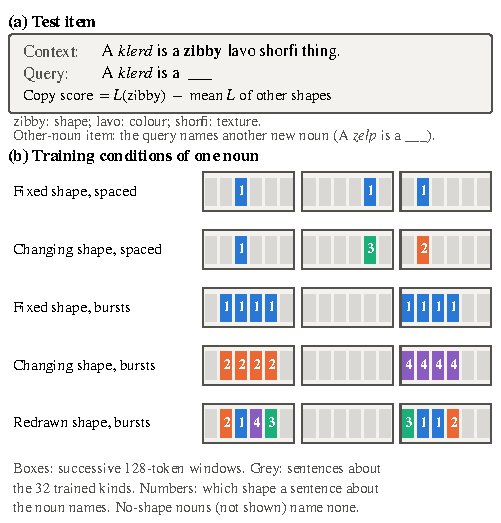
\includegraphics[width=\columnwidth]{figures/figure1_carry.pdf}
\caption{(a) A test item and the copy score, which leaves out the noun's own shape. (b) Training conditions (history and presentation), drawn schematically over three training windows. A burst puts four sentences in one window, so the same number of sentences fills a quarter as many windows. Redrawn-shape bursts are the control (Section~\ref{sec:bursts}); half-kept bursts and no-shape nouns are not shown.}
\label{fig:1}
\end{figure}

\section{Related Work}
\textbf{In-context and in-weights learning.} In-context learning emerges when items occur in bursts, more when their meanings change, and trades off against learning in the weights \citep{chan2022}; what is learned in context also generalises differently \citep{chan2022generalize}. It depends on task diversity \citep{raventos2023}, favours rare classes \citep{chan2025} and can fade as stored solutions take over \citep{singh2023}. Its onset has been traced to induction heads \citep{olsson2022,reddy2024}, and in small transformers stored bigram statistics are learned quickly and in-context ones later \citep{bietti2023}. Synthetic languages and Markov chains have been used to trace how in-context learning forms \citep{akyurek2024,edelman2024}. Resetting embeddings during training keeps in-context use alive for rare tokens \citep{anand2025}, and in models trained on synthetic biographies, balanced use of stored and in-context knowledge emerges only when facts repeat within a document, documents are moderately inconsistent and knowledge frequencies are skewed \citep{kim2026training}. We manipulate frequency, stored knowledge and presentation separately for single words within one model. By copying we mean the simplest form of in-context use: repeating a feature named in the previous sentence, as induction-style copying does, rather than learning a task from examples.

\textbf{Copying and recall.} Language models have long gained from copying recent words, through caches and pointers \citep{kuhn1990,grave2017,merity2017}, because words recur in bursts \citep{church1995,church2000,madsen2005}, a regularity that human memory also tracks \citep{anderson1991}. Pretrained models recall facts about frequent entities better than about rare ones \citep{mallen2023,kandpal2023}, their accuracy tracks how often terms occurred in pretraining \citep{razeghi2022}, and they vary in how far they follow contexts that contradict what they know \citep{longpre2021,xie2024,du2024}; recall of stored facts has been traced through specific pathways \citep{geva2023}, and copying and recall compete inside the network \citep{yu2023,jin2024,ortu2024}.

\textbf{New words and new tokens.} Rare and new words have poor representations \citep{schick2020}, and good embeddings for them can be built from a few contexts \citep{herbelot2017,khodak2018}; under-trained tokens behave abnormally \citep{land2024}, new embeddings are often initialised at the mean of existing ones \citep{hewitt2021}, and tying input and output embeddings \citep{press2017,inan2017} trains every token's embedding as an output. Lexical exposure can inflate apparent generalisation \citep{kim2022lexical}, and when language models acquire a word depends mainly on its frequency \citep{chang2022}. Children's word learning offers related evidence on shape \citep{landau1988,smith2002}, on expectations about how features vary \citep{kemp2007,dewar2010} and on the timing of exposures \citep{childers2002,schwab2016}, to which we return in Section~\ref{sec:discussion}.

\section{Setup}\label{sec:setup}\label{sec:background}
\textbf{Language.} Each corpus describes 32 kinds of object, each named by an invented noun (the \emph{trained kinds}), with 14 exemplars per kind. An exemplar has a shape, a colour and a texture, each one of ten invented words, and is described in one of five sentence frames that name the shape (and, in one sentence in fifteen, a frame that does not), such as \emph{A wug is a zibby lavo shorfi thing} (shape, colour, texture) or \emph{Look at the wug. It is zibby and lavo} (Appendix~\ref{app:lang}). The corpus runs through all exemplars many times, each pass arranged afresh, and a model reads it once. Sentences about a kind come in runs of four. In \textbf{stable-kind} corpora each kind keeps one shape, so its shape can be stored. In \textbf{shifting-kind} corpora a kind gets a new shape in every pass, so its current shape can come only from the context. Every word is one token.

\textbf{Models.} Decoder-only transformers with pre-layer normalisation and learned position embeddings, with 3.4M, 10.9M and 25.6M parameters (4 to 8 layers), and in Experiment~3 also 85.6M (12 layers), read the text once in windows of 128 tokens. All sizes reached a similar final training loss (0.39 to 0.40 nats per token). Sizes also differ in training steps, batch size, learning rate and amount of text (Appendix~\ref{app:train}), so differences between sizes are not a scaling trend. Input and output embeddings are untied, so a noun's input embedding carries everything the model has learned about the noun as an input; we also check tied embeddings.

\textbf{Controlling a noun's history.} We added 40 new nouns to each corpus. Four never occurred in training (\emph{unseen}); the other 36 did (\emph{familiar}). Each familiar noun had one history (Table~\ref{tab:design}) and a set number of sentences (\emph{exposures}), spread evenly from 5\% to 95\% of training, with three nouns per condition. Presented \emph{spaced}, a noun has one sentence per window. Presented in \emph{bursts}, it has four consecutive sentences in one window, like the trained kinds' runs. In \emph{mixed} corpora the familiar nouns are spread over all histories; in \emph{single-history} corpora all have changing shapes (\emph{changing-only}) or all fixed shapes (\emph{fixed-only}).

\begin{table}[t]
\centering
\small
\setlength{\tabcolsep}{3pt}
\begin{tabular}{@{}p{0.27\columnwidth}p{0.68\columnwidth}@{}}
\toprule
History & Sentences about the noun in training \\
\midrule
Unseen & none: the noun's embedding is untrained \\
Fixed shape & always the noun's own shape, which it can store \\
Changing shape & a new shape every sentence (spaced) or every burst (bursts), so nothing can be stored \\
No shape & no shape at all: the noun is familiar but has no shape to store \\
Redrawn shape & bursts only (control): a new shape every sentence, even within a burst \\
Half-kept shape & bursts only (control): each sentence keeps the previous shape half the time \\
\bottomrule
\end{tabular}
\caption{Noun histories. In changing-shape bursts the shape is shared within a burst and redrawn for each burst, so the noun's own earlier sentence is the only source of its current shape. In redrawn-shape bursts it matches only by chance.}
\label{tab:design}
\end{table}

\begin{table}[t]
\centering
\small
\setlength{\tabcolsep}{2.5pt}
\begin{tabular}{@{}l>{\raggedright\arraybackslash}p{0.50\columnwidth}lr@{}}
\toprule
Exp. & Nouns & Exposures & Models \\
\midrule
1 & fixed, changing, no shape; spaced & 10--10,000 & 90 \\
2 & the same; spaced and bursts & 100, 1,000 & 60 \\
3 & as Exp.~2, stable-kind only, new seeds; 85.6M models; single-history corpora & 100, 1,000 & 70 + 10$^t$ \\
C & changing, half-kept, redrawn and fixed bursts; spaced; Exp.~3's seeds & 100, 1,000 & 30 \\
P & with Exp.~2: Pythia, 22 real noun pairs, colour & -- & 5$^p$ \\
\bottomrule
\end{tabular}
\caption{Experiments. Experiments 1 and 2 used stable-kind and shifting-kind corpora (Experiment 1 also random-order corpora); Experiment 3 and the control (C) used stable-kind corpora only. $^t$Ten 3.4M models with tied embeddings (exploratory). $^p$Pretrained models, inference only (Section~\ref{sec:pythia}).}
\label{tab:exps}
\end{table}

\textbf{Measures.} A test item gives one sentence about a noun naming a shape $s$, then the start of the next mention, \emph{A \textit{noun} is a}, and reads the model's log probability $L$ of each of the ten shapes at the next position (Figure~\ref{fig:1}a). The \textbf{copy score} is $L(s)$ minus the mean of $L$ over the other shapes, leaving out the noun's own shape $s^*$, which the context never names (for nouns without a fixed shape, a shape assigned to the noun at random is left out, so every score compares $s$ with the same number of shapes). It is in nats: 3.4 means the context's shape is about 30 times as likely as the average other shape. Each noun gets 36 items. Because log probabilities share one normaliser, a stored shape that only raises its own probability leaves the copy score unchanged; the score falls only if the stored shape pushes the copied one down. So a low copy score for a fixed-shape noun is not a by-product of confidence in its stored shape. We therefore also report which shape the model prefers, the \textbf{output preference} $L(s^*) - L(s)$, and how strongly it has stored $s^*$: $L(s^*)$ minus the mean of the other shapes after an unrelated sentence (\textbf{stored preference}). In \textbf{other-noun items}, the query names another new noun with the same history; if copying is tied to the noun, these should score lower. We also score unseen nouns with a \textbf{typical embedding}: the mean of the trained kinds' embeddings plus a random offset of typical length.

\textbf{Predictions.} Table~\ref{tab:pred} gives what each account predicts. Only memory competition predicts that a stored shape lowers copying among spaced nouns. Useful context and recurrence both predict that changing-shape nouns copy more in bursts than spaced. Bursts might also help for two further reasons: the embedding is updated in fewer windows, and a test item, two consecutive sentences about one noun, resembles what burst nouns met in training and spaced nouns did not. Fixed-shape bursts share all of this, but their shape can be stored, so their context is not needed; memory competition predicts that they copy less only by as much as a stored shape lowers copying among spaced nouns. Redrawn-shape bursts recur and are updated like changing-shape bursts and store nothing, but their previous sentence is no guide, so only useful context predicts that changing-shape bursts copy more than they do.

\begin{table}[t]
\centering
\small
\setlength{\tabcolsep}{1.5pt}
\begin{tabular}{@{}>{\raggedright\arraybackslash}p{0.465\columnwidth}ccccl@{}}
\toprule
Comparison & Mem. & Rep. & Useful & Recur. & Exp. \\
\midrule
Unseen: typical $-$ untrained & & $<$0 & & & -- \\
Spaced: fixed $-$ changing & $<$0 & 0 & 0 & 0 & 3 \\
Changing: bursts $-$ spaced & 0 & 0$^b$ & $>$0 & $>$0 & 2, 3 \\
Bursts: changing $-$ fixed & $>$0$^c$ & 0$^b$ & $>$0 & 0 & 3 \\
Bursts: changing $-$ redrawn & 0 & 0 & $>$0 & 0 & C \\
Redrawn bursts $-$ spaced & 0 & 0$^b$ & 0 & $>$0 & C \\
\bottomrule
\end{tabular}
\caption{Predictions of the memory-competition, representation, useful-context and recurrence accounts for the copy score. Blank: no prediction. $^b$Or $>$0 if an embedding left less trained copies more. $^c$No larger than for spaced nouns. Exp.: experiments in which the comparison was a pre-registered test (C: the control, specified before training but not registered; --: exploratory only).}
\label{tab:pred}
\end{table}

\textbf{Experiments} (Table~\ref{tab:exps}). Experiment~1 asked whether familiarity alone ends copying, using spaced nouns from 10 to 10,000 exposures. Its nouns differed from the trained kinds in two ways: they never recurred within a window, and no-shape nouns never appeared in the test frame. Experiment~2 removed both differences (shaped nouns now appeared only in the test frame) and added bursts, at 100 and 1,000 exposures. Experiment~3 tested Experiment~2's findings on new models: ten new seeds at the three sizes, ten models of 85.6M parameters, and five seeds in single-history corpora. The \textbf{control} asked whether bursts keep copying because the noun recurs or because its context is useful. It kept Experiment~3's seeds and sizes and added \emph{redrawn-shape bursts}, whose shape is drawn anew for every sentence (the sentences of changing-shape spaced nouns, grouped in fours), and \emph{half-kept bursts}, in which each sentence keeps the previous shape with probability one half. Its design and predictions were fixed before training, but it was not registered. New nouns fill about 60\% of training windows in Experiment~1 and 8\% in Experiments~2 and~3 (40\% and 5\% for the 10.9M models), so we compare conditions only within an experiment.

\textbf{Analysis.} The seed is the unit: we average each condition over model sizes within a seed and test across seeds, with Holm correction within each registered family \citep{holm1979}, and count a prediction as supported only if its direction also holds in two of the three sizes. Experiments~1 to~3 were each registered before any of their models was trained; links to the time-stamped registrations are withheld for anonymous review, and the registered documents are in the supplementary material. These are all the experiments run with this design; earlier studies in the same language used other designs, and none of their data enter this paper. Appendix~\ref{app:reg} gives the registration history and every registered test with its outcome.

\section{Results}\label{sec:results}
Where Experiment~3 tested a comparison, we report its value; Table~\ref{tab:key} gives Experiment~2's beside it. Results not marked pre-registered are exploratory, including the control (specified before training but not registered), the mechanism analyses, tied embeddings and shifting-kind corpora.

\subsection{The Baseline: Unseen Nouns Copy, and Spaced Nouns Copy Less with Exposure}\label{sec:rows}
Experiment~1 set the baseline (Appendix~\ref{app:M}, Figure~\ref{fig:carry}). In stable-kind corpora unseen nouns copied 4.53 nats [95\% CI 3.54,~5.52], but because of their embeddings: given a typical embedding, the same nouns scored $-$0.33. Scaling an unseen noun's embedding to the trained kinds' average length, keeping its direction, lowered its score only by 0.52 nats, to 4.00 (pre-registered with Experiment~2 and supported, almost entirely at 3.4M; Table~\ref{tab:N5}); a random direction of that length kept copying (4.09), whereas the trained kinds' mean embedding removed it ($-$0.44). So direction, not length, matters. The same held in Experiment~3 (6.88 untrained, 0.79 typical) and with tied embeddings (3.96 and 0.02; ten 3.4M models, Appendix~\ref{app:O}).

\begin{figure*}[!t]
\centering
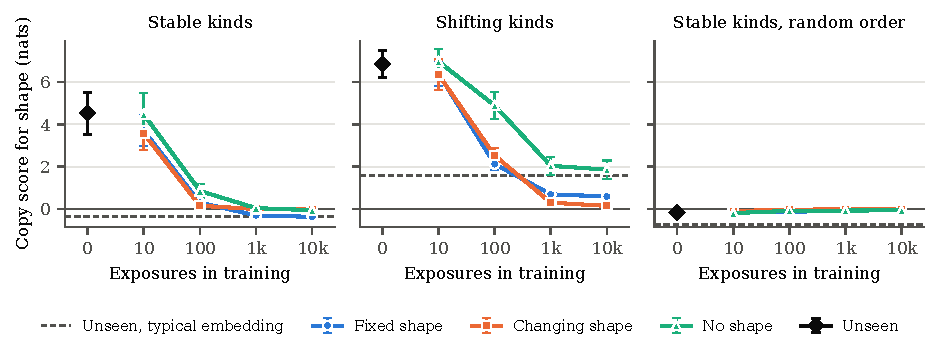
\includegraphics[width=0.92\textwidth]{figures/fig_a9_carry.pdf}
\caption{Experiment 1: copy score by number of exposures and noun history, all spaced, in stable-kind, shifting-kind and random-order corpora (means over ten seeds, sizes averaged; 95\% intervals). Diamond at 0: unseen nouns. Dashed line: unseen nouns with a typical embedding.}
\label{fig:carry}
\end{figure*}

In stable-kind corpora, familiar nouns met one sentence at a time copied less the more exposures they had had: 3.6--4.5 nats at 10 exposures, under 1 nat at 100, and between $-$0.37 and 0.05 at 1,000 and 10,000, whatever their history. Changing-shape nouns, with nothing to store, copied about as little as fixed-shape nouns, which stored their shape well (stored preference 9.5 nats at 1,000 exposures); the registered prediction that fixed-shape nouns would lose copying faster than no-shape nouns was not supported. In random-order corpora no noun copied, so the copying is learned from the runs of sentences about a kind: within a run the previous sentence names the kind's shape, so copying pays until the shape is stored, and the trained kinds themselves end up not copying ($-$0.02). In Experiment~2, unseen nouns' copying grew over training (Figure~\ref{fig:a10formation}): nothing in an untrained embedding turns off a tendency the model builds for all nouns. What, then, keeps it on for a familiar noun?

\subsection{Copying Stays High Only Where the Context Was Needed}\label{sec:bursts}
\textbf{Bursts with changing shapes copy.} Changing-shape bursts, where a noun's previous sentence gives its current shape and memory cannot, scored 4.14 nats [3.60,~4.69] more than changing-shape spaced nouns (pre-registered; Figure~\ref{fig:a11}a), as much at 1,000 exposures as at 100. At 1,000 exposures they scored 4.71 nats, against at most 1.1 for every other familiar history. The contrast was largest at 3.4M: at 25.6M the other histories kept 0.4 to 1.7 nats, against 3.56 (Table~\ref{tab:O2}). The comparison between 100 and 1,000 exposures is between different nouns at the end of training. Over training, copying for these nouns grew: in Experiment~2, nouns with 1,000 exposures went from 2.6, 1.1 and 0.8 nats at the first saved weights to 4.9, 3.3 and 3.3 at the end (3.4M, 10.9M, 25.6M), while fixed-shape bursts stayed between 0.2 and 1.3 (Figure~\ref{fig:a10formation} shows the average over sizes).

\begin{table*}[!t]
\centering\small

\setlength{\tabcolsep}{3pt}
\begin{tabular}{@{}lllrrrrrl@{}}
\toprule
Corpus & History & Exp. & 3.4M & 10.9M & 25.6M & 85.6M & Mean$^a$ & 95\% CI$^a$ \\
\midrule
Mixed & Unseen & -- & 8.96 & 6.03 & 5.65 & 6.96 & 6.88 & [6.31, 7.45] \\
 & Fixed, spaced & 100 & 1.10 & 1.53 & 2.10 & 1.29 & 1.58 & [1.34, 1.82] \\
 & Fixed, spaced & 1,000 & 0.36 & 0.64 & 0.39 & 0.30 & 0.46 & [0.27, 0.65] \\
 & Fixed, bursts & 100 & 6.17 & 3.76 & 4.36 & 5.12 & 4.76 & [4.18, 5.35] \\
 & Fixed, bursts & 1,000 & 0.69 & 1.09 & 1.32 & 0.67 & 1.03 & [0.83, 1.23] \\
 & No shape, spaced & 100 & 2.59 & 2.93 & 4.03 & 3.98 & 3.18 & [2.68, 3.68] \\
 & No shape, spaced & 1,000 & \textminus{}0.02 & 0.92 & 1.67 & 0.91 & 0.86 & [0.56, 1.15] \\
 & No shape, bursts & 100 & 3.16 & 4.66 & 5.27 & 5.81 & 4.36 & [3.76, 4.96] \\
 & No shape, bursts & 1,000 & 0.06 & 1.55 & 1.54 & 1.16 & 1.05 & [0.80, 1.30] \\
 & Changing, spaced & 100 & 1.63 & 2.12 & 2.17 & 2.18 & 1.97 & [1.63, 2.32] \\
 & Changing, spaced & 1,000 & 0.28 & 0.63 & 0.79 & 0.36 & 0.57 & [0.42, 0.71] \\
 & Changing, bursts & 100 & 9.03 & 4.53 & 4.77 & 5.55 & 6.11 & [5.57, 6.66] \\
 & Changing, bursts & 1,000 & 7.05 & 3.53 & 3.56 & 4.85 & 4.71 & [4.03, 5.40] \\
\midrule
Changing only & Unseen & -- & 9.01 & 5.15 & 4.33 & -- & 6.16 & [4.25, 8.08] \\
 & Changing, spaced & 100 & 1.65 & 2.20 & 1.37 & -- & 1.74 & [0.96, 2.52] \\
 & Changing, spaced & 1,000 & 0.43 & 1.55 & 0.83 & -- & 0.94 & [0.44, 1.44] \\
 & Changing, bursts & 100 & 9.33 & 4.80 & 3.72 & -- & 5.95 & [4.09, 7.81] \\
 & Changing, bursts & 1,000 & 9.23 & 4.39 & 3.00 & -- & 5.54 & [4.12, 6.96] \\
\midrule
Fixed only & Unseen & -- & 7.22 & 3.31 & 4.09 & -- & 4.87 & [3.84, 5.90] \\
 & Fixed, spaced & 100 & 0.18 & 1.05 & 1.26 & -- & 0.83 & [0.71, 0.95] \\
 & Fixed, spaced & 1,000 & \textminus{}0.16 & 0.11 & 0.08 & -- & 0.01 & [\textminus{}0.10, 0.12] \\
 & Fixed, bursts & 100 & 1.68 & 1.55 & 2.09 & -- & 1.77 & [1.26, 2.29] \\
 & Fixed, bursts & 1,000 & \textminus{}0.23 & 0.31 & 0.00 & -- & 0.03 & [\textminus{}0.13, 0.18] \\
\bottomrule
\end{tabular}

\caption{Experiment 3: copy score by corpus design, history and exposures (means over seeds by size, and seed-level mean with 95\% interval, sizes averaged). Mixed: ten seeds; single-history designs: five seeds. $^a$Over the three smaller sizes, as in the registered tests; 85.6M models were trained in the mixed design only.}
\label{tab:O2}
\end{table*}

\textbf{Not because bursts leave embeddings less trained.} Fixed-shape bursts have the same frame, presentation and number of updates, but a shape that memory can supply. Presentation in bursts by itself added little: fixed-shape bursts copied only 0.57 nats [0.39,~0.74] more than fixed-shape spaced nouns at 1,000. Changing-shape bursts copied 3.68 nats [2.99,~4.37] more than fixed-shape bursts at 1,000 exposures, in the same direction at all three sizes (pre-registered): 6.36, 2.44 and 2.24 nats at 3.4M, 10.9M and 25.6M. In ten models of 85.6M the difference was 4.18 [2.95,~5.41] (pre-registered). Those models also had a longer warm-up and other hardware, and sizes differ in more than size, so we do not read the pattern across sizes as a trend. With tied embeddings (3.4M, exploratory) the pattern held but was weaker: changing-shape bursts copied 4.29 nats at 1,000 exposures, 1.90 [1.20,~2.60] more than fixed-shape bursts, while the other familiar histories kept 1.4 to 2.9 nats.

\textbf{Not because the noun recurs.} In the control, redrawn-shape bursts recur as changing-shape bursts do, but their previous sentence names the current shape only by chance (one time in ten). At 1,000 exposures they copied 0.49 nats, no more than changing-shape spaced nouns (0.07 [$-$0.01,~0.15] above them), and 3.33 [2.74,~3.92] less than changing-shape bursts in the same models, in all ten seeds and at every size (5.82, 2.04 and 2.14 nats; Figure~\ref{fig:a11}b, Table~\ref{tab:P1}). Half-kept bursts fell in between (1.20 nats), so copying rose with how often the previous sentence was right. Recurrence helped only nouns met less often: at 100 exposures redrawn-shape bursts copied 0.96 nats [0.76,~1.15] more than spaced nouns, as no-shape bursts did (pre-registered in Experiment~2, levels pooled), whose gain at 1,000 was 0.05 in Experiment~2 and 0.20 [$-$0.10,~0.49] in Experiment~3. The control also replicated the main contrast: changing-shape bursts copied 3.01 [2.42,~3.59] more than fixed-shape bursts. It used Experiment~3's seeds with new corpora, so it is not fully independent of it.

\begin{table*}[!t]
\centering\small

\begin{tabular}{@{}lrrrr@{}}
\toprule
& \multicolumn{2}{c}{100 exposures} & \multicolumn{2}{c}{1,000 exposures} \\
\cmidrule(lr){2-3}\cmidrule(lr){4-5}
History & Mean & 95\% CI & Mean & 95\% CI \\
\midrule
Changing, bursts & 4.09 & [3.68, 4.49] & 3.82 & [3.21, 4.44] \\
Half-kept, bursts & 2.99 & [2.57, 3.40] & 1.20 & [0.92, 1.47] \\
Redrawn, bursts & 2.28 & [1.94, 2.62] & 0.49 & [0.41, 0.58] \\
Fixed, bursts & 3.18 & [2.75, 3.62] & 0.82 & [0.68, 0.95] \\
Changing, spaced & 1.32 & [1.11, 1.54] & 0.42 & [0.38, 0.47] \\
Fixed, spaced & 1.22 & [1.07, 1.37] & 0.39 & [0.32, 0.46] \\
\midrule
\multicolumn{5}{@{}l}{\emph{Differences}} \\
Bursts: changing $-$ redrawn & 1.81 & [1.33, 2.30] & 3.33 & [2.74, 3.92] \\
Bursts: changing $-$ half-kept & 1.10 & [0.70, 1.50] & 2.63 & [2.13, 3.12] \\
Bursts: half-kept $-$ redrawn & 0.71 & [0.36, 1.05] & 0.71 & [0.46, 0.95] \\
Redrawn bursts $-$ changing spaced & 0.96 & [0.76, 1.15] & 0.07 & [\textminus{}0.01, 0.15] \\
Bursts: redrawn $-$ fixed & \textminus{}0.91 & [\textminus{}1.38, \textminus{}0.43] & \textminus{}0.32 & [\textminus{}0.47, \textminus{}0.18] \\
Bursts: changing $-$ fixed & 0.90 & [0.58, 1.22] & 3.01 & [2.42, 3.59] \\
\bottomrule
\end{tabular}

\caption{Control: copy score by condition and paired differences (nats; seed-level means over ten seeds, sizes averaged within seed; t-based 95\% intervals).}
\label{tab:P1}
\end{table*}

\textbf{Without nouns of the other history.} In single-history corpora no noun of another history was present (Figure~\ref{fig:a11}c). There, changing-shape bursts copied 5.51 nats [4.24,~6.78] more than fixed-shape bursts at 1,000 exposures, at all three sizes (pre-registered), so the main difference does not need nouns of the other history. It was larger than in mixed corpora with the same seeds (4.27), because fixed-shape bursts lost all their copying when no noun of another history shared the corpus: 0.03 nats against 1.03, a difference of 1.00 [0.80,~1.20] (pre-registered). For changing-shape bursts this comparison was inconclusive. Unseen nouns' copying also varied with the corpus: 4.87 [3.84,~5.90] in fixed-only corpora, 6.16 [4.25,~8.08] in changing-only and 7.35 in mixed corpora with the same five seeds, and 4.92 in the control's corpora against 6.88 in Experiment~3's on the same ten seeds. So a noun's copying depends on which other nouns share the corpus, not only on its own history.

\begin{table}[t]
\centering
\small
\setlength{\tabcolsep}{2.2pt}
\begin{tabular}{@{}l@{\hspace{1pt}}rrrr@{}}
\toprule
& \multicolumn{2}{c}{Exp.~2} & \multicolumn{2}{c}{Exp.~3} \\
\cmidrule(lr){2-3}\cmidrule(l){4-5}
Comparison & Pooled & 1,000 & Pooled & 1,000 \\
\midrule
Changing: bursts $-$ spaced & 3.39$^r$ & 3.35 & 4.14$^r$ & 4.15 \\
Bursts: changing $-$ fixed & 1.73 & 2.86 & 2.52 & 3.68$^r$ \\
No shape: bursts $-$ spaced & 0.80$^r$ & 0.05 & 0.69 & 0.20 \\
Spaced: fixed $-$ changing & $-$0.02 & 0.02 & $-$0.25$^r$ & $-$0.10 \\
Spaced: fixed $-$ no shape$^a$\! & $-$1.02$^r$ & $-$0.46 & $-$1.00 & $-$0.39 \\
Same noun $-$ other noun & 0.05 & 0.05 & 0.07 & 0.08$^r$ \\
Beyond geometry & & 2.84 & & 3.67$^r$ \\
\midrule
\multicolumn{3}{@{}l}{\emph{Control models}} & Pooled & 1,000 \\
Bursts: changing $-$ redrawn & & & 2.57 & 3.33 \\
Redrawn bursts $-$ spaced & & & 0.51 & 0.07 \\
Bursts: changing $-$ fixed & & & 1.96 & 3.01 \\
\bottomrule
\end{tabular}
\caption{Key comparisons in stable-kind corpora (copy score, nats; seed-level means; 100 and 1,000 exposures pooled, and 1,000 alone). $^r$The value that was the pre-registered test (pooled or at 1,000, as registered); all other values exploratory. Intervals for the registered values are in Tables~\ref{tab:N1} and~\ref{tab:O1}. Same noun $-$ other noun: other-noun items, for changing-shape bursts. Beyond geometry: changing-shape bursts relative to the copying predicted from their embeddings' geometry (Section~\ref{sec:kept}). $^a$Confounded with expected word class. Control models: Exp.~3's seeds, new corpora; spaced means changing-shape spaced; specified before training, not registered.}
\label{tab:key}
\end{table}

\begin{figure*}[t]
\centering
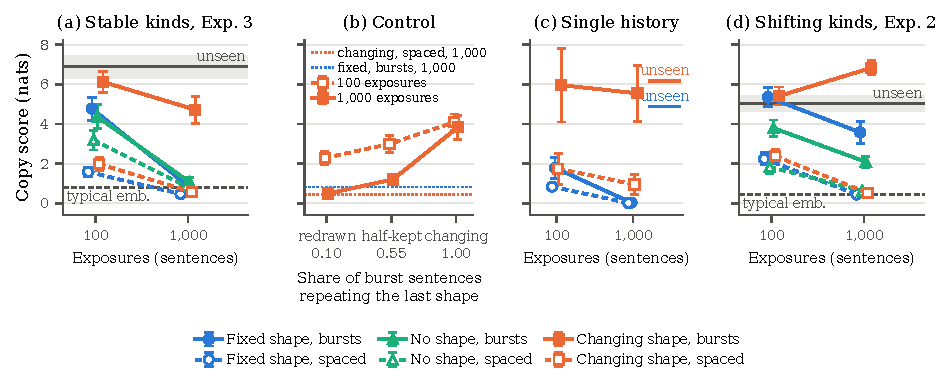
\includegraphics[width=\textwidth]{figures/fig_a11.pdf}
\caption{Copy score at 100 and 1,000 exposures (means over seeds, sizes averaged; 95\% intervals; points offset for legibility). In (a), (c) and (d), colour shows history and line style presentation (solid: bursts; dashed: spaced). Nouns at 100 and 1,000 exposures are different nouns, all scored at the end of training; lines join conditions, not time points. (a) Stable-kind corpora, Experiment~3 (ten new seeds). (b) Control: copy score of redrawn, half-kept and changing-shape bursts against how often a burst sentence repeats the previous one's shape (dashed: 100 exposures; solid: 1,000), with changing-shape spaced nouns and fixed-shape bursts at 1,000 as dotted reference lines. (c) Single-history corpora, Experiment~3 (five seeds): all familiar nouns have changing shapes (orange) or all have fixed shapes (blue). (d) Shifting-kind corpora, Experiment~2 (exploratory). Solid grey line and band: unseen nouns; dashed line: unseen nouns with a typical embedding. Experiment~2's stable-kind results are in Figure~\ref{fig:a10}.}
\label{fig:a11}
\end{figure*}

\subsection{A Stored Shape Wins in Prediction but Barely Lowers Copying}\label{sec:memory}
\textbf{At test.} Fixed- and changing-shape spaced nouns share frame, presentation and expected word class, and differ only in whether a shape can be stored. Fixed-shape spaced nouns copied 0.25 nats [0.15,~0.35] less (pre-registered), mostly at 100 exposures (0.40) rather than 1,000 (0.10): the stored shape pushed the copied one down a little (the registered equivalence test against $\pm$0.3 nats was inconclusive; \citealp{lakens2017}). In prediction, however, the stored shape won, which the copy score cannot register by design: fixed-shape spaced nouns preferred their own shape to the context's by 5.84 nats [5.57,~6.11] (pre-registered). Fixed-shape spaced nouns also scored about 1 nat below no-shape spaced nouns (pre-registered in Experiment~2), but no-shape nouns expect a colour where the others expect a shape, so this difference reflects word class.

\textbf{In training.} Spaced nouns copy little (under 2 nats), so the test above has little to suppress. Three comparisons do not depend on it. First, at 1,000 exposures a stored shape lowered spaced nouns' copying by 0.10 nats, but the burst difference was 3.58 nats [2.94,~4.22] larger; even a proportional suppression (about a fifth) would predict a burst difference of about 0.9. Second, bursts that stored nothing still lost their copying: no-shape bursts copied no more than fixed-shape bursts (1.05 against 1.03), and redrawn-shape bursts in the control copied less (0.49 against 0.82). Third, in tied models a stored shape did not lower spaced nouns' copying at all ($-$0.01). (Bursts stored the shape less well than spaced presentation only at 100 exposures: 3.0 against 5.4 nats in Experiment~2.) On this evidence, what a storable shape changed was which nouns kept copying after training: copying stayed high only where the context had been needed. Memory was not manipulated during training, so this is an inference from these comparisons.

\subsection{What Is Kept, and Where}\label{sec:kept}
\textbf{A tendency, mostly not a link.} If changing-shape bursts bound a noun to its current shape, other-noun items should score lower. They did, but by only 0.08 nats [0.02,~0.14] at 1,000 exposures, within $\pm$0.3 (pre-registered), and no other condition in mixed or fixed-only corpora exceeded 0.14: the model copied the latest shape after the query noun, whichever noun the context described. Training never required it to check, since a burst never contains a sentence about another noun. In changing-only corpora, where every familiar noun's context was useful, changing-shape bursts showed a larger noun-specific part (0.33 nats [0.18,~0.48], five seeds).

\textbf{The query noun's history matters more.} With a context about a noun of one history and a query naming another, the query noun's history mattered more than the context noun's (1.72 against 0.47 nats for changing- versus fixed-shape bursts; difference 1.25 [0.94,~1.56], pre-registered).

\textbf{What in the embedding carries it.} All other weights are shared, so a difference between nouns in one model must enter through their input embeddings. Is it a simple property, such as how far the embedding has moved? Not on three measures. Within each model we regressed copy scores on each familiar noun's embedding's cosine with its initial value, its distance from the trained kinds' mean and its norm: at 1,000 exposures changing-shape bursts copied 3.67 nats [3.03,~4.32] more than these three measures predict (pre-registered), although their embeddings were only slightly closer to their initial values than those of fixed-shape bursts (cosine 0.85 against 0.78). This rules out these three summaries, not geometry in general. Three exploratory analyses go further (Appendix~\ref{app:O}). Part of the tendency lies along a direction shared by nouns: adding the difference between the mean embeddings of changing- and fixed-shape bursts, taken from other nouns, raised copying at 1,000 exposures by 1.51 nats [1.20,~1.82] for fixed-shape spaced nouns and 1.99 for unseen nouns with a typical embedding, while a random vector of the same length changed it by at most 0.02 (Table~\ref{tab:O4}). The direction mattered most at 3.4M (2.41 for fixed-shape spaced nouns, against 1.12 and 1.00 at 10.9M and 25.6M), and subtracting it from changing-shape bursts at 25.6M changed nothing (+0.02), so outside 3.4M it carries a minority of the effect. Patching hidden states \citep{zhang2024patching} showed that by the end of the second block the difference between histories had passed from the query noun's position to the position where the shape is predicted, as a readout through attention would require. At that position, attention in the first block to the context's shape word tracked copying within each model (mean Spearman $\rho$ = 0.80 [0.76,~0.85]). In the first block the query noun can change this attention only through its own key, by competing in the softmax; the correlation does not show that this is how it acts. A registered head search in Experiment~1 found no induction-like heads (Appendix~\ref{app:M}).

\begin{table*}[!t]
\centering\small

\begin{tabular}{@{}llrlrl@{}}
\toprule
Nouns & Baseline & Direction & 95\% CI & Random & 95\% CI \\
\midrule
Fixed, spaced & 0.46 & 1.51 & [1.20, 1.82] & \textminus{}0.02 & [\textminus{}0.11, 0.08] \\
Changing, spaced & 0.57 & 1.06 & [0.76, 1.36] & \textminus{}0.01 & [\textminus{}0.06, 0.04] \\
No shape, spaced & 0.86 & 2.04 & [1.58, 2.49] & \textminus{}0.01 & [\textminus{}0.16, 0.13] \\
No shape, bursts & 1.05 & 3.06 & [2.45, 3.67] & 0.02 & [\textminus{}0.16, 0.19] \\
Unseen, typical embedding & 0.79 & 1.99 & [1.55, 2.44] & \textminus{}0.02 & [\textminus{}0.24, 0.19] \\
Fixed, bursts$^a$ & 1.03 & 0.99 & [0.53, 1.44] & 0.07 & [\textminus{}0.04, 0.19] \\
Changing, bursts$^b$ & 4.71 & \textminus{}0.82 & [\textminus{}1.37, \textminus{}0.28] & \textminus{}0.30 & [\textminus{}0.59, \textminus{}0.01] \\
\bottomrule
\end{tabular}

\caption{Experiment 3, steering (exploratory): copy score with the noun's own embedding (baseline; typical embedding for unseen nouns) and change when the changing-minus-fixed burst direction from other nouns, or a random vector of the same length, is added to the embedding (nats; ten seeds, sizes averaged). Nouns at 1,000 exposures. $^a$Direction from 100-exposure bursts. $^b$Direction from 100-exposure bursts subtracted.}
\label{tab:O4}
\end{table*}

\subsection{When the Whole Corpus Rewards Copying}\label{sec:beyond}
All results so far come from corpora whose trained kinds keep their shapes. What if they do not? In Experiment~2's shifting-kind corpora, where the trained kinds' shapes can come only from context, nouns of every history in bursts kept copying (Figure~\ref{fig:a11}d): at 1,000 exposures fixed-shape bursts scored 3.57 nats, no-shape bursts 2.09 and changing-shape bursts 6.82, more than unseen nouns (5.02). Fixed-shape and no-shape bursts still copied less at 1,000 exposures than at 100 (5.35 and 3.79), while changing-shape bursts copied more (5.40 at 100). So how much copying a familiar noun keeps depends on the corpus: where the trained kinds themselves reward copying, every history in bursts keeps some, and the gap between changing- and fixed-shape bursts remains (3.25 nats).


\subsection{Beyond the Artificial Language}\label{sec:pythia}
A registered test in five Pythia models (1B to 12B; \citealp{biderman2023}) found no consistent effect of replacing 22 pairs of real nouns' embeddings with typical or untrained-scale ones (colour; Appendix~\ref{app:N}). In WikiText-103 (introduced by \citealp{merity2017}) those nouns recur in bursts (24 to 40\% of mentions followed by another within 128 words, against under 1\% expected), and a colour named twice within one article usually agrees (median 0.86 to 0.98) while two mentions from anywhere agree less (0.37 to 0.46; exploratory, Appendix~\ref{app:O}): in this respect natural text resembles changing-shape bursts.


\section{Discussion}\label{sec:discussion}
\textbf{What decides copying.} In stable-kind corpora the model builds a tendency to copy the latest shape and, through each noun's embedding, keeps it where the previous sentence was needed. Of the four accounts, memory competition at prediction explains little (at most 0.4 nats in any experiment); representation is right that the difference enters through the embedding, but history mattered beyond simple measures of its geometry; recurrence alone did not keep copying. Useful context fits best, and on our inference memory acts through it: where a shape could be stored, the context was not needed during training.

\textbf{What this adds.} \citet{chan2022} showed that bursty items whose meaning changes favour in-context learning across a population of items. We find the same rule acting on single words within one model; the model can do this because each word has its own embedding, but nothing forces it to. Three results go further: memory's effect appears to fall on training rather than prediction; what is kept is a tendency to copy, mostly not tied to the noun, whose size depends on the other nouns in the corpus; and usefulness, not recurrence, keeps copying, in graded form. The lower copying of nouns met more often is a per-word counterpart of the transience of in-context learning, which fades as training continues \citep{singh2023}. \citet{anand2025} keep in-context use alive by resetting embeddings; we find that use carried by each word's embedding. \citet{kim2026training} trace the balance of stored and in-context knowledge to repetition and inconsistency within documents and to skewed frequencies; we find comparable factors acting on single words and separate frequency from whether anything can be stored.

\textbf{Implications.} For evaluation: in small models trained from scratch, a probe with invented words can measure the untrained embedding more than anything learned about context, so effects should be checked against a typical embedding, itself an intervention; in pretrained models with subword tokens, where our Pythia test found no embedding effect, this caution may not transfer. For new tokens: in our models, a token added with a mean-like embedding behaves like a familiar word that does not copy, whereas a randomly initialised one copies. For knowledge conflicts: whether a model follows the context for a word may depend on whether the context was needed for that word in training, not only on how often the word occurred. Tests of in-context use should therefore report how the probe words occurred in training.

\textbf{Analogies with children.} As analogies only: changing-shape bursts resemble the boxes of \citet{dewar2010}, uniform within and varying between, from which 9-month-olds formed an overhypothesis in the sense of \citet{kemp2007}, expecting the next draw to match; and spaced nouns stored their shape better at 100 exposures while bursts kept the context in use, as children retain words and categories better from spaced exposures \citep{childers2002,vlach2008} but learn labels repeated in successive sentences \citep{schwab2016}.

\section{Limitations}
\textbf{Language and scale.} The language is artificial, with 32 kinds, three features, single-token words and five sentence frames; the models are small (at most 85.6M parameters), with one training recipe per size. Sizes differ in steps, batch, learning rate and amount of text; the effect was largest at 3.4M, and the 85.6M models had a longer warm-up and other hardware. With tied embeddings (one size, added after the results), familiar nouns kept more copying. \textbf{Design.} Experiments~2 and~3 tested 100 and 1,000 exposures; comparisons across exposures are between different nouns, and exposure count is confounded with exposure rate and, over training, with training time. Test items for fixed-shape nouns pit the context against the stored shape, while those for changing-shape nouns do not. No-shape comparisons are confounded with expected word class, and the test of memory competition rests on spaced nouns, which copied little. The learned copying is narrow: with one unrelated sentence between context and query it almost vanished (at most 0.44 nats), with the context in another frame changing-shape bursts kept 38 to 40\% of it, and no noun copied colour, which varies within every kind. A typical embedding suppresses copying even in shifting-kind corpora, where the trained kinds copy strongly, so it may be atypical in its own way. \textbf{Status of analyses.} The control was not registered (its design and predictions were fixed before training) and reused Experiment~3's seeds with three repeat rates. The mechanism, tied-embedding and shifting-kind analyses were added after the results, and the heads involved were not identified. Single-history corpora used five seeds; planned power for a 1-nat difference in Experiment~1 was 0.57. \textbf{Checks beyond the language.} The pretrained test used one model family, 22 noun pairs and colour only, and the WikiText-103 counts include many names (\emph{Black Sea}). Earlier experiments in this language, not reported here, were registered in stages (Appendix~\ref{app:reg}).

\section{Ethics and Use of AI Assistants}
All training data are artificial; the pretrained models are public. No data were collected from people. Code, registrations and results are provided as anonymised supplementary material; every corpus can be rebuilt exactly from the code, and the trained models will be released with the paper.

An AI assistant (Claude, Anthropic) was used to help design analyses, write code, review code and design, draft and edit text and check citations. It also reviewed the write-up of Experiment~1, which identified the two differences addressed by Experiment~2, and coded the colour typicality of the pretrained-model nouns in two independent passes. The authors are responsible for all content, including the accuracy of every citation.

\bibliography{refs}
\bibliographystyle{nejlt_bib}

\clearpage
\appendix
\onecolumn
\let\oldsection\section
\renewcommand{\section}{\clearpage\oldsection}
\FloatBarrier
\appendixsection{Language and Corpora}\label{app:lang}
\setcounter{table}{0}\renewcommand{\thetable}{\thesection\arabic{table}}
\setcounter{figure}{0}\renewcommand{\thefigure}{\thesection\arabic{figure}}
\textbf{Language.} Each corpus describes 32 kinds of object, each named by an invented noun, with 14 exemplars per kind. Each exemplar has a shape, a colour and a texture, each an invented word from a list of ten, and is described by one sentence in one of five frames:
\begin{enumerate}[itemsep=0pt,topsep=2pt]
\item \emph{A wug is a [shape] [colour] [texture] thing.}
\item \emph{Look at the wug. It is [shape] and [colour].}
\item \emph{Here is another wug. This one is [shape].}
\item \emph{The wug I showed you is [shape], but a different [colour].}
\item \emph{That is a wug because it is [shape].}
\end{enumerate}
Shape is named in all five frames, colour in three and texture in one. In one sentence in fifteen the trained kinds also appear in a frame without a shape (New nouns, below). The 448 sentences of a corpus make up one pass. Every word is one token of a byte-pair tokeniser with 329 entries, shared by all models.

\textbf{Order and kinds.} Within each pass the sentences about each kind are shuffled, cut into runs of four and the runs shuffled across kinds (grouped order). In stable-kind corpora each kind keeps one shape across its exemplars, while colour and texture vary. In shifting-kind corpora each kind receives a new shape, drawn at random, in every pass and keeps it within the pass. Experiment~1 also used stable-kind corpora in random order, with every pass shuffled.

\textbf{Text read.} Each model read fresh text once, in non-overlapping 128-token windows in a fixed order: 160,000 windows for the 3.4M, 25.6M and 85.6M models and 256,000 for the 10.9M models, which share the rules and nouns of the shorter corpus. Each pass is arranged with its own random draw.

\textbf{New nouns.} Forty new nouns per corpus, three per condition and four unseen, rotated over nouns across seeds. A noun's sentences (its exposures) were placed evenly between 5\% and 95\% of the windows read, at most one unit (a sentence, or a burst of four) per window, between the trained kinds' runs, at a random position in the window. In Experiment~1 fixed- and changing-shape nouns appeared in frames 1 to 5 and no-shape nouns in a sixth frame, \emph{The [noun] is [colour] and [texture]}, which the trained kinds also used in one sentence in fifteen. In Experiments~2 and~3 fixed- and changing-shape nouns appeared only in frame 1 and no-shape nouns only in \emph{A [noun] is a [colour] [texture] thing}, which the trained kinds used in one sentence in fifteen. A checker re-read every corpus and verified exposures, units, frames, shapes within bursts and window placement; all corpora matched checksums recorded before training.

\FloatBarrier
\appendixsection{Models and Training}\label{app:train}
\setcounter{table}{0}\renewcommand{\thetable}{\thesection\arabic{table}}
Decoder-only transformers with pre-layer normalisation, learned position embeddings, GELU feed-forward layers, AdamW (betas 0.9 and 0.95, weight decay 0.1), linear warm-up then cosine decay, and dropout 0.1 (Table~\ref{tab:train}). Input and output embeddings are untied: the output layer starts as a copy of the input embedding and is trained separately, and every final model was checked to have different input and output matrices (on why, see Appendix~\ref{app:reg}). Final training loss was similar across sizes: in Experiment~3, 0.40, 0.39, 0.39 and 0.39 nats per token at 3.4M, 10.9M, 25.6M and 85.6M (range over models 0.37 to 0.42). The ten tied-embedding models of Appendix~\ref{app:O} were trained on other hardware, with input and output embeddings sharing one matrix; all ten final models were checked after training, and in each the two matrices were identical. Models of Experiments~1 and~2 and the three smaller sizes of Experiment~3 were trained on one AMD graphics card (DirectML); the 85.6M and tied models on an Apple M3 Ultra.

\begin{table}[!htbp]
\centering\small

\begin{tabular}{@{}lrrrr@{}}
\toprule
Setting & 3.4M & 10.9M & 25.6M & 85.6M \\
\midrule
Layers, heads, width & 4, 4, 256 & 6, 8, 384 & 8, 8, 512 & 12, 12, 768 \\
Feed-forward width & 1,024 & 1,536 & 2,048 & 3,072 \\
Steps & 5,000 & 8,000 & 10,000 & 10,000 \\
Batch & 32 & 32 & 16 & 16 \\
Peak learning rate & $3\times10^{-4}$ & $2\times10^{-4}$ & $1\times10^{-4}$ & $1\times10^{-4}$ \\
Warm-up steps & 200 & 400 & 500 & 1,000 \\
\bottomrule
\end{tabular}
\caption{Model and training settings. Batches are of 128-token windows.}
\label{tab:train}
\end{table}

\textbf{Data and code.} All code, corpora, test items, scores and analysis outputs, and the final weights and training logs of every model, will be released on publication; anonymised copies of the code and results are in the supplementary material, with the command that regenerates each table and figure.

\FloatBarrier
\appendixsection{Registrations, Terms and Registered Tests}\label{app:reg}
\setcounter{table}{0}\renewcommand{\thetable}{\thesection\arabic{table}}
\textbf{Registrations.} All registrations are in one public project on the Open Science Framework (link withheld for review). The project began with earlier studies of this language (a set of training experiments, an analysis of natural corpora and a test of pretrained models), registered in stages, some after related results were known; they are not reported here. During that work we found that the earlier models' embeddings had not been tied as intended (the tie was lost on the graphics hardware used) and that a loading error had changed their scores; both were corrected and disclosed in the registrations. We therefore chose untied embeddings for this paper and checked every model. The three experiments of this paper were registered as amendments. Experiment~1 was registered before its corpora were built. Experiment~2, with the embedding analysis and the pretrained test, was registered after Experiment~1's results and after its corpora were built, before any of its models was trained or any pretrained model was run on its items. Experiment~3 was registered after all of Experiment~2's results, including the exploratory analyses that it tests, and before any of its models was trained (Appendix~\ref{app:O}). The control (Appendix~\ref{app:P}) was not registered; its design and predictions were committed to the project repository before training. Each registration states what was known when it was written. The registrations use other names for the conditions (Table~\ref{tab:terms}).

\begin{table}[!htbp]
\centering\small

\begin{tabular}{@{}ll@{}}
\toprule
Main text & Registrations \\
\midrule
Experiment 1 & Amendment 9 (the familiarity study) \\
Experiment 2 & Amendment 10, Part A \\
Embedding analysis of Experiment 1 (Section~\ref{sec:rows}) & Amendment 10, Part C \\
Pretrained test (Appendix~\ref{app:N}) & Amendment 10, Part B \\
Experiment 3 & Amendment 11 (Parts A, B and C) \\
Stable-kind corpora & Regular (grouped) corpora \\
Shifting-kind corpora & Reassigned (grouped) corpora \\
Single-history corpora (changing-only, fixed-only) & pure\_changing, pure\_fixed \\
Spaced, bursts & singles, runs \\
Changing shape & uninformative (Experiment 1), rotating (Experiments 2 and 3) \\
No shape & shape-absent, absent \\
Redrawn-shape, half-kept bursts (control) & redrawn\_run, half\_run (not registered) \\
Other-noun items & noun\_specific (same minus other noun) \\
Output preference & compete \\
Copy score & carry \\
Stored preference & knowledge \\
Embedding & row \\
Typical embedding & typical row \\
Random embedding of untrained scale & atypical\_init \\
\bottomrule
\end{tabular}
\caption{Main-text terms and the terms used in the registrations.}
\label{tab:terms}
\end{table}

\textbf{Registered tests.} Table~\ref{tab:hyp} lists every registered hypothesis of the three experiments, the embedding analysis and the pretrained test, with its outcome under the registered decision rules (Holm correction within each registered family; direction in at least two of three model sizes; for the pretrained test, Holm within each model and support in at least four of five models). Equivalence bounds were set in each registration: $\pm$1 nat in Experiment~1 (about one seventh of the fall from unseen to typical embeddings in earlier work in this language); in Experiment~2, $\pm$0.3 nats for H40, H41 and H44 (the smallest history effect in Experiment~1), $\pm$1 nat for the check K1, and the larger of 0.3 nats and one fifth of a pilot effect for H48; in Experiment~3, $\pm$0.3 nats for H52, H54 and H59.

\begin{table}[!htbp]
\centering\small

\begin{tabular}{@{}lp{0.50\textwidth}p{0.33\textwidth}@{}}
\toprule
Label & Prediction (main-text terms) & Outcome \\
\midrule
\multicolumn{3}{@{}l}{\emph{Experiment 1 (Amendment 9)}} \\
M1 & Fixed-shape nouns store their shape (stored preference $>$ 0.2 nats at 1,000 exposures, rising) & Passed in all three corpora \\
H30 & Copying falls faster with exposure for fixed-shape than no-shape nouns & Not supported (wrong direction) \\
H31 & No-shape nouns (1,000 and 10,000) differ from unseen nouns with a typical embedding; equivalence $\pm$1 & Different (0.33) and equivalent \\
H32 & Fixed-shape nouns' preference for their own shape, measured in the copy items, rises with exposure & Supported \\
H33 & Ablating candidate heads removes more than half of unseen nouns' copying, more than random heads & Not supported \\
H34 & Ablating candidate heads lowers trained kinds' copying in shifting-kind corpora & Supported; random heads cut it nearly as much \\
H35 & Candidate heads' attention falls faster for fixed-shape nouns & Not tested (required H33) \\
R1 & Unseen nouns copy more in grouped than random order & Replicated \\
\addlinespace
\multicolumn{3}{@{}l}{\emph{Experiment 2 (Amendment 10, Part A); stable-kind corpora}} \\
M2 & Unseen nouns copy more than 1 nat & Passed \\
K1 & Fixed-shape nouns' stored preference equal ($\pm$1) in bursts and spaced & Not equivalent: H41 not interpreted \\
H40 & No-shape: bursts differ from spaced; equivalence $\pm$0.3 & Bursts higher \\
H41 & Fixed shape: bursts differ from spaced; equivalence $\pm$0.3 & Bursts higher (not interpreted) \\
H42 & Changing shape: bursts copy more than spaced & Supported \\
H43 & Spaced: fixed shape copies less than no shape & Supported; confounded by expected word class \\
H44 & Spaced no-shape nouns differ from unseen nouns with a typical embedding; equivalence $\pm$0.3 & Higher; not equivalent \\
\addlinespace
\multicolumn{3}{@{}l}{\emph{Experiment 3 (Amendment 11); stable-kind corpora; Holm over H50--H53, H55, H56}} \\
M3 & Unseen nouns copy more than 1 nat & Passed \\
H50 & At 1,000: changing-shape bursts copy more than fixed-shape bursts (primary) & Supported (3.68) \\
H51 & Changing shape: bursts copy more than spaced & Supported (4.14) \\
H52 & Spaced: fixed differs from changing shape; equivalence $\pm$0.3 & Fixed lower (\textminus{}0.25); not equivalent \\
H53 & Fixed-shape spaced nouns prefer their own shape to the context's & Supported (5.84) \\
H54 & Noun-specific copying of changing-shape bursts within $\pm$0.3 & Within $\pm$0.3 (0.08) \\
H55 & Changing-shape bursts copy more than embedding geometry predicts & Supported (3.67) \\
H56 & The query noun's history matters more than the context noun's & Supported (1.25) \\
M3B, H57 & 85.6M models: unseen nouns copy; changing-shape bursts copy more than fixed-shape bursts & Passed; supported (4.18) \\
M3C & Single-history corpora: unseen nouns copy & Passed \\
H58 & Changing-shape bursts (changing-only) copy more than fixed-shape bursts (fixed-only) & Supported (5.51) \\
H59 & Single-history minus mixed corpora, same history; equivalence $\pm$0.3 & Changing bursts inconclusive; fixed bursts lower (\textminus{}1.00) \\
\addlinespace
\multicolumn{3}{@{}l}{\emph{Embedding analysis (Amendment 10, Part C); Experiment 1 models}} \\
H49 & Scaling unseen nouns' embeddings to the trained kinds' norm lowers copying & Supported (driven by the 3.4M models) \\
\addlinespace
\multicolumn{3}{@{}l}{\emph{Pretrained models (Amendment 10, Part B)}} \\
H45 & A random embedding of untrained scale raises copying over the own embedding & Not supported (2 of 5 models) \\
H46 & The same embedding raises copying over a typical embedding & Not supported (2 of 5 models) \\
H47 & Colour-typical nouns copy less than colour-variable nouns & Not supported (0 of 5) \\
H48 & The H45 increase differs between colour-typical and colour-variable nouns & Inconclusive \\
\bottomrule
\end{tabular}
\caption{Registered hypotheses and outcomes. Full statistics: Tables~\ref{tab:M1} (Experiment 1), \ref{tab:N1} (Experiment 2), \ref{tab:N5} (embedding analysis), \ref{tab:N6} (pretrained models) and \ref{tab:O1} (Experiment 3). Candidate heads (H33 to H35): in each Experiment~1 model, the heads with the highest product of prefix-matching and copying scores (Table~\ref{tab:M4}).}
\label{tab:hyp}
\end{table}

\FloatBarrier
\section{Experiment 1 (Amendment 9)}\label{app:M}
\setcounter{table}{0}\renewcommand{\thetable}{\thesection\arabic{table}}
\setcounter{figure}{0}\renewcommand{\thefigure}{\thesection\arabic{figure}}
\textbf{Registration.} The design, hypotheses and analysis were registered before any corpus was built (Amendment 9). An addendum, written the same day before any corpus was built, fixed details the registration left open (36 context draws per noun; uniform frame proportions; exposures placed at evenly spaced read positions from 5\% to 95\% of training, after warm-up for every size; random in-window position; the 40 new nouns; how the pilot fixes the number of nouns per cell; how a hypothesis counts as supported; the gate for H35; and that heads without prefix matching are described as copying heads). A pilot (one seed, 3.4M models, never used in a test) set three nouns per cell; with the registered rule the expected power for a 1-nat difference was 0.57, below the planned 0.8, which we report as a shortfall. Corpus checksums were recorded before training and matched on the training machine; a checker verified every exposure, window and frame from the tokens. All models were trained on one machine.

\textbf{Design.} In every model, 40 new nouns fill 13 cells (three per cell, four unseen): fixed shape, changing shape (a new shape in every sentence, drawn from the corpus's shape distribution) and no shape (a sixth frame, \emph{The \textit{noun} is \textit{colour} and \textit{texture}}, also used by trained kinds in one sentence in fifteen), each at 10, 100, 1,000 and 10,000 exposures, plus unseen. Nouns rotate over cells across ten seeds. Each familiarity sentence lies wholly inside one 128-token window, at most one per window, between runs in grouped corpora. Base corpora: stable-kind, stable-kind random-order, shifting-kind; sizes 3.4M, 10.9M and 25.6M; ten seeds; 90 models with untied embeddings. Measures are read from the full log-softmax over the ten shape words at the position that predicts the shape in \emph{A \textit{noun} is a}: copy score $= L(s) - \bar L$ after a context sentence with shape $s$; own-shape preference $= L(s^*) - \bar L$; stored preference $= L(s^*)$ minus the mean over the other nine shapes after an unrelated sentence, where $\bar L$ is the mean over shapes other than $s$ and $s^*$.

\begin{table}[!htbp]
\centering\small

\begin{tabular}{@{}lp{0.27\textwidth}rrrcp{0.17\textwidth}@{}}
\toprule
& Test & Estimate & 95\% CI & Holm $p$ & Sizes & Verdict \\
\midrule
M1 & Stored preference at 1,000 exposures, fixed shape (each corpus) & 9.53; 8.61; 8.26 & & & & Passed \\
H30 & Copy score falls faster with exposure for fixed-shape than no-shape nouns (slope difference) & 0.16 & [0.01, 0.30] & 1.000 & 0 & Not supported \\
H31 & No shape (1k and 10k) minus unseen with typical embedding (two-sided; TOST $\pm$1) & 0.33 & [0.13, 0.52] & .013 & 3 & Different, and equivalent within 1 nat \\
H32 & Own-shape preference rises with exposure, fixed shape (slope) & 2.97 & [2.79, 3.16] & $<$.001 & 3 & Supported \\
H33a & Ablating candidates removes more than half of unseen copy score (proportion) & 0.22 & [0.07, 0.36] & 1.000 & 2 & Not supported \\
H33b & Random heads minus candidates, unseen copy score after ablation & 0.64 & [\textminus{}0.43, 1.71] & 1.000 & 2 & Not supported \\
H34 & Shifting-kind: trained-kind copy score intact minus candidates ablated & 7.41 & [6.02, 8.80] & $<$.001 & 3 & Supported \\
H35 & Attention slope, fixed shape minus no shape & 0.002 & [\textminus{}0.000, 0.005] & -- & 2 & Not tested (gate) \\
R1 & Replication: stable-kind minus random-order corpora, unseen copy score & 4.68 & [3.71, 5.65] & $<$.001$^a$ & 3 & Replicated \\
\bottomrule
\end{tabular}
\\[2pt]{\footnotesize $^a$ Outside the Holm family (replication); unadjusted one-sided $p$. M1 values: stable-kind; stable-kind random-order; shifting-kind (all with slopes above zero, $p<.001$). H31 TOST $p<.001$.}
\caption{Registered tests of the familiarity study (stable-kind models unless stated; seed-level estimates over ten seeds, sizes averaged within seed; nats, proportions for H33a, attention probability for H35). Holm $p$ is adjusted over H30 to H34; H35 was not entered because H33(a) failed. Sizes: number of the three model sizes with the registered direction.}
\label{tab:M1}
\end{table}

\begin{table}[!htbp]
\centering\small

\begin{tabular}{@{}lrrrlrrrr@{}}
\toprule
Corpus & Unseen & Typical & Trained & Familiar nouns & 10 & 100 & 1k & 10k \\
\midrule
Stable-kind & 4.53 & \textminus{}0.33 & \textminus{}0.02 & Fixed shape & 3.70 & 0.30 & \textminus{}0.30 & \textminus{}0.37 \\
 & & & & Changing shape & 3.57 & 0.16 & 0.00 & \textminus{}0.01 \\
 & & & & No shape & 4.47 & 0.86 & 0.05 & \textminus{}0.05 \\
\addlinespace
Shifting-kind & 6.85 & 1.57 & 9.98 & Fixed shape & 6.40 & 2.13 & 0.70 & 0.60 \\
 & & & & Changing shape & 6.34 & 2.53 & 0.30 & 0.15 \\
 & & & & No shape & 6.97 & 4.89 & 2.04 & 1.86 \\
\addlinespace
Stable-kind random-order & \textminus{}0.15 & \textminus{}0.72 & \textminus{}0.10 & Fixed shape & \textminus{}0.13 & \textminus{}0.13 & \textminus{}0.06 & \textminus{}0.05 \\
 & & & & Changing shape & \textminus{}0.10 & \textminus{}0.03 & \textminus{}0.02 & \textminus{}0.01 \\
 & & & & No shape & \textminus{}0.19 & \textminus{}0.09 & \textminus{}0.07 & \textminus{}0.05 \\
\bottomrule
\end{tabular}
\caption{Copy score (nats) by noun type and exposure, mean of seed values (sizes averaged). Unseen: never in training; typical: the unseen nouns with a typical embedding; trained: the 32 trained kinds.}
\label{tab:M2}
\end{table}

\begin{table}[!htbp]
\centering\small

\begin{tabular}{@{}llrrrr@{}}
\toprule
Type & Measure & 10 & 100 & 1k & 10k \\
\midrule
Fixed shape & Stored preference & 1.59 & 8.02 & 9.53 & 10.61 \\
 & Own shape & 1.41 & 7.74 & 9.56 & 10.71 \\
Changing shape & Stored preference & 0.04 & \textminus{}0.03 & 0.00 & 0.03 \\
 & Own shape & 0.01 & \textminus{}0.03 & \textminus{}0.01 & 0.03 \\
No shape & Stored preference & \textminus{}0.14 & \textminus{}0.17 & 0.12 & 0.08 \\
 & Own shape & 0.11 & \textminus{}0.16 & 0.10 & 0.06 \\
\bottomrule
\end{tabular}
\caption{Stored preference and own-shape preference (nats) in stable-kind models, mean of seed values.}
\label{tab:M3}
\end{table}

\begin{table}[!htbp]
\centering\small

\begin{tabular}{@{}llrrrrrrrrr@{}}
\toprule
 & & & & \multicolumn{3}{c}{Unseen copy score} & \multicolumn{3}{c}{Trained copy score} & \\
\cmidrule(lr){5-7}\cmidrule(lr){8-10}
Corpus & Size & $k$ & Prefix & Intact & Cand. & Random & Intact & Cand. & Random & DLA \\
\midrule
Stable-kind & 3.4M & 2 & 0.028 & 8.10 & \textminus{}0.42 & 5.26 & \textminus{}0.25 & \textminus{}0.85 & \textminus{}0.71 & \textminus{}0.04 \\
 & 10.9M & 4 & 0.037 & 2.98 & 5.80 & 1.95 & 0.08 & 0.17 & \textminus{}0.40 & \textminus{}0.01 \\
 & 25.6M & 6 & 0.037 & 2.50 & 0.73 & 0.81 & 0.12 & \textminus{}0.60 & \textminus{}0.18 & \textminus{}0.01 \\
Shifting-kind & 3.4M & 2 & 0.029 & 6.48 & 4.22 & 3.27 & 9.59 & 2.83 & 3.37 & \textminus{}0.12 \\
 & 10.9M & 4 & 0.032 & 7.21 & 6.56 & 4.82 & 10.10 & 5.02 & 2.45 & \textminus{}0.03 \\
 & 25.6M & 6 & 0.031 & 6.88 & 0.26 & 3.26 & 10.26 & \textminus{}0.11 & 3.39 & \textminus{}0.01 \\
Stable-kind random-order & 3.4M & 2 & 0.028 & \textminus{}0.24 & \textminus{}0.09 & \textminus{}0.34 & \textminus{}0.08 & 0.00 & \textminus{}0.11 & \textminus{}0.01 \\
 & 10.9M & 4 & 0.030 & 0.04 & 0.25 & 0.03 & \textminus{}0.06 & 0.04 & \textminus{}0.11 & \textminus{}0.01 \\
 & 25.6M & 6 & 0.030 & \textminus{}0.25 & 0.00 & \textminus{}0.37 & \textminus{}0.18 & \textminus{}0.10 & \textminus{}0.27 & \textminus{}0.01 \\
\bottomrule
\end{tabular}
\caption{Head analysis by corpus and size (means over ten seeds). Candidates were the $k$ heads with the highest product of prefix-matching and copying scores; in grouped models they were in layer 0 in all but one model (a 3.4M stable-kind model chose one layer-1 head), and in random-order models a few were in later layers. In the 3.4M and 10.9M models layer 0 has exactly $k$ non-candidate heads, so the random draws repeat one set. Prefix: highest prefix-matching score of any head (uniform attention gives about 0.027). Copy score of unseen nouns and of trained kinds intact, with the candidates mean-ablated, and with random heads ablated (mean of 200 or 20 draws). DLA: change in unseen copy score predicted by the candidates' direct paths. In stable-kind 10.9M models, ablating the candidates raised unseen nouns' copying (2.98 to 5.80); we have no explanation for this.}
\label{tab:M4}
\end{table}




\begin{figure}[!htbp]
\centering
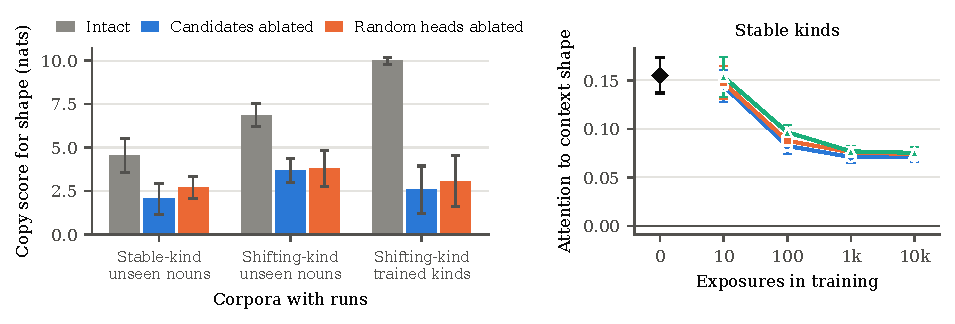
\includegraphics[width=\textwidth]{figures/fig_a9_heads.pdf}
\caption{Experiment 1. Left: copy score intact, with the candidate heads mean-ablated, and with random heads ablated (nats; mean over ten seeds and three sizes, 95\% intervals over seeds). Right: the candidates' attention from the position that predicts the shape to the context's shape word, stable-kind models (exploratory).}
\label{fig:heads}
\end{figure}



\FloatBarrier
\section{Experiment 2, the Embedding Analysis and the Pretrained Test (Amendment 10)}\label{app:N}
\setcounter{table}{0}\renewcommand{\thetable}{\thesection\arabic{table}}
\setcounter{figure}{0}\renewcommand{\thefigure}{\thesection\arabic{figure}}
\textbf{Registration.} Amendment 10 has three parts: Experiment 2 (Part A), the pretrained test (Part B) and the embedding analysis of the Experiment 1 models (Part C). It was registered after the Amendment 9 results, after its corpora were built and checksummed, and before any of them was used, any of its models was trained, or any pretrained model was run on its items. It answered two confounds raised by a blind review of the Amendment 9 results (by an AI assistant given only the write-up of Experiment 1): new nouns never recurred within a window, and no-shape nouns never appeared in a frame with a shape slot after \emph{is a}. The noun lists for the pretrained test were fixed, with checksums, before the pilot. A pilot on Pythia-410M (never in a test) gave a mean increase of 0.13 nats from the original to the random (untrained scale) embedding, so the smallest effect of interest for H48 was 0.30 nats by the registered rule. One deviation: some Pythia tokenizers define no padding token, so the scoring script falls back to token id 0; padded positions are masked and only the last real token is read, and batched and single-item scores agreed exactly. No score had been produced by the affected models.

\textbf{Experiment 2 design.} Everything not stated is as in Amendment 9 (Appendix~\ref{app:M}). Histories: \emph{fixed shape}, frame 1 (\emph{A \textit{noun} is a \textit{shape} \textit{colour} \textit{texture} thing}) with the noun's own shape; \emph{no shape}, frame 7 (\emph{A \textit{noun} is a \textit{colour} \textit{texture} thing}), which names no shape; \emph{changing-shape}, frame 1 with a shape drawn from the corpus's shape distribution, a new one for every sentence when presented spaced and one per burst, redrawn for each burst, when presented in bursts. Presentation: \emph{spaced}, one sentence per unit; \emph{bursts}, four consecutive sentences about the noun in one window. Exposures (100 or 1,000) count sentences, so bursts and spaced nouns are matched in sentences, not in units or spacing. Trained kinds use frame 7 in one sentence in fifteen, so the frame is not new. Three nouns per cell (12 cells) and four unseen nouns; stable-kind (confirmatory) and shifting-kind (exploratory) base corpora; three sizes and ten seeds (60 models). A checker re-read every corpus and verified exposures, units, frames, shapes within bursts and window placement; all 40 corpora matched checksums recorded before training.

\begin{table}[!htbp]
\centering\small

\begin{tabular}{@{}lp{0.34\textwidth}rrrcp{0.17\textwidth}@{}}
\toprule
& Test & Estimate & 95\% CI & Holm $p$ & Sizes & Reading \\
\midrule
M2 & Unseen copy score minus 1 nat (manipulation check) & 5.35 & [4.59, 6.12] & $<$.001$^a$ &  & Passed \\
K1 & Stored preference, fixed-shape bursts minus fixed-shape spaced nouns (equivalence $\pm$1) & \textminus{}1.09 & [\textminus{}1.45, \textminus{}0.73] & $<$.001$^a$ &  & Not equivalent (H41 not interpreted) \\
H40 & No-shape bursts minus no-shape spaced nouns (two-sided; TOST $\pm$0.3) & 0.80 & [0.47, 1.13] & $<$.001 & 3 & Above \\
H41 & Fixed-shape bursts minus fixed-shape spaced nouns (two-sided; TOST $\pm$0.3) & 1.69 & [1.29, 2.08] & $<$.001 & 3 & Above (not interpreted) \\
H42 & Changing-shape bursts minus changing-shape spaced nouns (one-sided) & 3.39 & [2.69, 4.09] & $<$.001 & 3 & Supported \\
H43 & Fixed-shape spaced nouns minus no-shape spaced nouns (one-sided) & \textminus{}1.02 & [\textminus{}1.27, \textminus{}0.76] & $<$.001 & 3 & Supported \\
H44 & No-shape spaced nouns minus unseen with typical embedding (two-sided; TOST $\pm$0.3) & 1.42 & [1.12, 1.73] & $<$.001 & 3 & Above \\
\bottomrule
\end{tabular}
\\[2pt]{\footnotesize $^a$ Outside the Holm family; unadjusted $p$. The M2 estimate is unseen copy score minus 1 nat, so unseen copy score was 6.35 nats.}
\caption{Registered tests of Experiment 2 (stable-kind models; 100 and 1,000 exposures pooled; seed-level estimates over ten seeds, sizes averaged within seed; nats). Holm $p$ is adjusted over H40 to H44. Sizes: number of the three sizes with the estimate's direction. Readings follow the registered table: ``above'' means the Holm threshold was met and the direction held at two of three sizes; TOST $p$ for H40, H41 and H44 was above .99, so none was equivalent.}
\label{tab:N1}
\end{table}

\begin{table}[!htbp]
\centering\small

\begin{tabular}{@{}llll@{}}
\toprule
Corpora & Noun & 100 exposures & 1,000 exposures \\
\midrule
Stable kinds & Fixed shape, spaced & 1.52 {[}1.18, 1.86{]} & 0.52 {[}0.36, 0.69{]} \\
 & Fixed shape, bursts & 4.43 {[}3.49, 5.36{]} & 0.99 {[}0.68, 1.30{]} \\
 & No shape, spaced & 3.09 {[}2.56, 3.63{]} & 0.98 {[}0.76, 1.20{]} \\
 & No shape, bursts & 4.65 {[}3.94, 5.36{]} & 1.03 {[}0.59, 1.47{]} \\
 & Changing shape, spaced & 1.59 {[}1.30, 1.88{]} & 0.50 {[}0.38, 0.62{]} \\
 & Changing shape, bursts & 5.02 {[}4.18, 5.86{]} & 3.85 {[}2.93, 4.77{]} \\
 & Unseen & 6.35 {[}5.59, 7.12{]} &  \\
 & Unseen, typical embedding & 0.61 {[}0.28, 0.95{]} &  \\
\midrule
Shifting kinds & Fixed shape, spaced & 2.23 {[}1.92, 2.55{]} & 0.44 {[}0.37, 0.51{]} \\
 & Fixed shape, bursts & 5.35 {[}4.88, 5.82{]} & 3.57 {[}3.02, 4.11{]} \\
 & No shape, spaced & 1.83 {[}1.49, 2.17{]} & 0.63 {[}0.53, 0.72{]} \\
 & No shape, bursts & 3.79 {[}3.38, 4.20{]} & 2.09 {[}1.82, 2.35{]} \\
 & Changing shape, spaced & 2.37 {[}2.04, 2.71{]} & 0.51 {[}0.38, 0.64{]} \\
 & Changing shape, bursts & 5.40 {[}4.95, 5.86{]} & 6.82 {[}6.48, 7.17{]} \\
 & Unseen & 5.02 {[}4.61, 5.42{]} &  \\
 & Unseen, typical embedding & 0.43 {[}0.32, 0.55{]} &  \\
\bottomrule
\end{tabular}
\caption{Copy score (nats) by cell, mean of seed values (sizes averaged) with 95\% intervals over ten seeds. Unseen nouns have no exposures; the typical embedding replaces an unseen noun's input embedding with one typical of trained nouns.}
\label{tab:N2}
\end{table}

\begin{table}[!htbp]
\centering\small

\begin{tabular}{@{}lrrrr@{}}
\toprule
 & \multicolumn{2}{c}{Stored preference} & \multicolumn{2}{c}{Slot} \\ \cmidrule(lr){2-3}\cmidrule(lr){4-5}
Noun & 100 & 1,000 & 100 & 1,000 \\
\midrule
Fixed shape, spaced & 5.37 & 7.80 & 4.03 & 6.16 \\
Fixed shape, bursts & 3.02 & 7.98 & 3.28 & 6.24 \\
No shape, spaced & 0.00 & \textminus{}0.09 & \textminus{}2.98 & \textminus{}4.93 \\
No shape, bursts & 0.05 & \textminus{}0.25 & \textminus{}1.12 & \textminus{}4.43 \\
Changing shape, spaced & \textminus{}0.08 & 0.01 & 5.04 & 5.30 \\
Changing shape, bursts & 0.14 & 0.06 & 3.74 & 5.24 \\
\bottomrule
\end{tabular}
\caption{Stored preference of the noun's own shape and expectation of a shape rather than a colour at the query position (slot: log of the summed probability of the ten shapes minus that of the ten colours), stable-kind models, mean of seed values (exploratory). Unseen nouns: stored preference \textminus{}0.04, slot 1.49.}
\label{tab:N3}
\end{table}





\textbf{Embedding geometry of the Experiment 2 models (exploratory, added after the results).} For every familiar noun in the 60 final models we recorded its input embedding's cosine with its initial embedding (rebuilt from the seed; the rebuild reproduced the unseen nouns' embeddings, which receive no gradient, in every model), its distance from the trained kinds' mean embedding and its norm; the copy score with its own embedding, with a typical embedding and with the embedding of a noun of another history (embeddings swapped between changing- and fixed-shape bursts and between changing-shape bursts and spaced nouns); the copy score with one sentence about a trained kind between context and query (gap), with the context in the frame \emph{Look at the \textit{noun}. It is \textit{shape} and \textit{colour}.} (other frame), and for the context's colour after \emph{A \textit{noun} is a \textit{shape}} (colour); and first-block attention from the query position to the context's shape, averaged over heads. Full results, including shifting-kind corpora and 100 exposures, are in the supplementary material.

\begin{table}[!htbp]
\centering\small

\begin{tabular}{@{}lrrrrrrr@{}}
\toprule
Noun & Own embedding & Typical embedding & Gap & Other frame & Colour & Cos.\ initial & Attention \\
\midrule
Unseen & 6.35 &  & 0.16 & 4.38 & \textminus{}0.30 & 1.000 & 0.186 \\
Fixed, spaced & 0.52 & 0.67 & 0.05 & 0.12 & \textminus{}0.10 & 0.732 & 0.089 \\
Fixed, bursts & 0.99 & 0.61 & 0.13 & 0.32 & \textminus{}0.12 & 0.778 & 0.099 \\
No shape, spaced & 0.98 & 0.63 & \textminus{}0.04 & 0.71 & \textminus{}0.22 & 0.793 & 0.102 \\
No shape, bursts & 1.03 & 0.68 & \textminus{}0.07 & 0.66 & \textminus{}0.34 & 0.806 & 0.097 \\
Changing, spaced & 0.50 & 0.61 & 0.10 & 0.20 & \textminus{}0.10 & 0.794 & 0.108 \\
Changing, bursts & 3.85 & 0.66 & 0.37 & 1.53 & \textminus{}0.12 & 0.849 & 0.168 \\
\bottomrule
\end{tabular}
\caption{Experiment 2 embedding geometry, stable-kind corpora, 1,000 exposures (unseen nouns: no exposures). Copy scores in nats; cosine of the embedding with its initial value; first-block attention from the query to the context's shape. Seed-level means. Swapping embeddings between changing- and fixed-shape bursts moved the copying with the embedding (2.88 nats [2.01, 3.76] and 2.88 [1.99, 3.76] in the two directions; since all other weights are shared, this mainly confirms that the difference enters through the embedding). In a noun-level regression of the copy score on embedding geometry (cosine with the initial embedding, distance from the trained kinds' mean, norm, size and seed; standard errors clustered by seed), changing-shape bursts scored 3.19 nats [2.46, 3.91] more than geometry predicts at 1,000 exposures and $-$0.09 [$-$0.51, 0.33] at 100. With the per-model regression registered for Experiment~3 (coefficient averaged over sizes within seed; Table~\ref{tab:key}), 2.84 [1.97, 3.70] at 1,000 and 0.15 [$-$0.29, 0.58] at 100.}
\label{tab:N13}
\end{table}

\begin{table}[!htbp]
\centering\footnotesize\setlength{\tabcolsep}{4pt}

\begin{tabular}{@{}lrrrrrrr@{}}
\toprule
Context $\backslash$ query & \shortstack{Unseen} & \shortstack{Fixed\\ spaced} & \shortstack{Fixed\\ bursts} & \shortstack{No shape\\ spaced} & \shortstack{No shape\\ bursts} & \shortstack{Changing\\ spaced} & \shortstack{Changing\\ bursts} \\
\midrule
Unseen & 6.34 & 0.60 & 0.73 & 1.16 & 1.01 & 0.42 & 2.61 \\
Fixed, spaced & 3.67 & 0.62 & 0.75 & 0.94 & 0.93 & 0.44 & 1.73 \\
Fixed, bursts & 5.14 & 0.68 & 1.01 & 1.07 & 1.27 & 0.53 & 2.45 \\
No shape, spaced & 4.10 & 0.53 & 0.74 & 1.12 & 1.13 & 0.39 & 1.67 \\
No shape, bursts & 4.30 & 0.62 & 0.91 & 0.89 & 1.01 & 0.43 & 2.07 \\
Changing, spaced & 4.03 & 0.59 & 0.91 & 1.26 & 1.12 & 0.50 & 1.86 \\
Changing, bursts & 6.49 & 0.85 & 1.15 & 1.49 & 1.39 & 0.66 & 3.80 \\
\bottomrule
\end{tabular}
\caption{Crossed histories (exploratory), stable-kind corpora, 1,000 exposures (unseen nouns: none): copy score when the context sentence is about a noun of one history (rows) and the query names a different noun of another (columns); 24 items per pair and model, seed-level means. Averaged over familiar histories, a queried noun with changing-shape bursts copied 1.35 nats [0.97, 1.74] more than one with fixed-shape bursts, and a context noun with changing-shape bursts raised copying by 0.39 [0.19, 0.58]. Full results are in the supplementary material.}
\label{tab:N14}
\end{table}

\textbf{The embedding analysis (Experiment 1 models).} In the 60 final grouped models of Amendment 9 we replaced the input embeddings of unseen nouns and computed the copy score again; the unmodified condition reproduced the Amendment 9 scores. Conditions: own embedding; own direction scaled to the mean norm of the trained kinds' embeddings (own direction, trained norm); a random direction at that norm (random direction, trained norm); the trained kinds' mean embedding. No-shape nouns at 10,000 exposures were also scored with their own direction scaled to the unseen nouns' mean norm (own direction, unseen norm).

\begin{table}[!htbp]
\centering\small

\begin{tabular}{@{}lrrrrrr@{}}
\toprule
 & \multicolumn{4}{c}{Unseen nouns} & \multicolumn{2}{c}{No shape, 10k} \\ \cmidrule(lr){2-5}\cmidrule(lr){6-7}
Corpus & Own & \shortstack{Own dir.,\\trained norm} & \shortstack{Random dir.,\\trained norm} & Trained mean & Own & \shortstack{Own dir.,\\unseen norm} \\
\midrule
Stable-kind & 4.53 & 4.00 & 4.09 & \textminus{}0.44 & \textminus{}0.05 & 0.53 \\
Shifting-kind & 6.85 & 7.12 & 7.15 & 1.05 & 1.86 & 4.16 \\
\bottomrule
\end{tabular}
\caption{The embedding analysis: copy score (nats) by input embedding, mean over seeds (sizes averaged). H49 (registered, stable-kind): own direction at trained norm minus own \textminus{}0.52 [\textminus{}0.85, \textminus{}0.20], one-sided $p$ = .003, direction at 2 of 3 sizes, supported. In shifting-kind models the same contrast went the other way (0.27 [0.12, 0.41]; exploratory). Random minus own direction, both at trained norm: 0.09 (stable-kind), 0.03 (shifting-kind).}
\label{tab:N5}
\end{table}

\textbf{The pretrained test.} 44 nouns in 22 pairs, matched on Pile frequency and count/mass type, were coded for colour typicality by two independent AI passes with a fixed prompt before any model was run (exact agreement 94\%, weighted $\kappa$ = 0.96); nouns that are also colour terms or that both passes flagged as polysemous were excluded. Colour-typical nouns are mostly natural kinds, so kind was a covariate. Each noun was read in three neutral frames with each of the eleven basic colour terms that are one token; copy score is the mean over frames and ordered colour pairs of $\log p(c_1 \mid c_1) - \log p(c_1 \mid c_2)$, with colour probabilities renormalised over the colour set. Only the noun's input embedding was changed.

\begin{table}[!htbp]
\centering\small

\begin{tabular}{@{}lrrrrrrrr@{}}
\toprule
 & \multicolumn{2}{c}{H45} & \multicolumn{2}{c}{H46} & \multicolumn{2}{c}{H47} & \multicolumn{2}{c}{H48} \\ \cmidrule(lr){2-3}\cmidrule(lr){4-5}\cmidrule(lr){6-7}\cmidrule(lr){8-9}
Model & Est. & Holm & Est. & Holm & Est. & Holm & Est. & TOST $p$ \\
\midrule
1B & 0.20 & met & 0.21 & met & 0.00 & -- & 0.07 & .097 \\
1.4B & 0.34 & met & \textminus{}0.22 & -- & \textminus{}0.01 & -- & \textminus{}0.08 & .021 \\
2.8B & \textminus{}0.38 & -- & 0.08 & -- & \textminus{}0.16 & -- & 0.11 & .222 \\
6.9B & 0.07 & -- & 0.36 & met & \textminus{}0.09 & -- & 0.10 & .127 \\
12B & \textminus{}0.35 & -- & \textminus{}0.21 & -- & 0.11 & -- & 0.08 & .066 \\
\bottomrule
\end{tabular}
\\[2pt]{\footnotesize Mixed model over the five primary models (copy score $\sim$ condition $\times$ group + model + kind; random intercepts for noun and pair, random condition slopes by noun): random (untrained scale) 0.00 ($p$ = .956), typical embedding \textminus{}0.04 ($p$ = .559), colour-variable group 0.06 ($p$ = .527).}
\caption{Registered tests in the pretrained models, by primary model (nouns or pairs as units; Holm within model over H45 to H48). H45: random (untrained scale) minus original; H46: random (untrained scale) minus typical embedding; H47: colour-typical minus colour-variable nouns, original embeddings; H48: difference between groups in the H45 increase (TOST against $\pm$0.30). A hypothesis needed Holm in at least four of the five models. Outcome: H45 and H46 met Holm in two of five models, H47 in none, and H48 was inconclusive (equivalent in one model).}
\label{tab:N6}
\end{table}

\begin{table}[!htbp]
\centering\small

\begin{tabular}{@{}lrrrrrrr@{}}
\toprule
Model & Original & \shortstack{Random,\\untrained scale} & \shortstack{Random,\\own scale} & Typical & \shortstack{Colour-\\typical} & \shortstack{Colour-\\variable} & \shortstack{Prior\\entropy} \\
\midrule
70M & 1.59 & 1.40 & 1.41 & 1.16 & 1.61 & 1.56 & 2.09 \\
160M & 0.93 & 1.95 & 1.95 & 1.03 & 0.87 & 1.00 & 2.01 \\
1B & 1.89 & 2.09 & 2.09 & 1.88 & 1.89 & 1.89 & 1.95 \\
1.4B & 2.10 & 2.44 & 2.44 & 2.66 & 2.10 & 2.10 & 1.97 \\
2.8B & 2.70 & 2.31 & 2.31 & 2.23 & 2.61 & 2.78 & 1.92 \\
6.9B & 2.67 & 2.75 & 2.75 & 2.39 & 2.63 & 2.72 & 1.94 \\
12B & 2.68 & 2.33 & 2.33 & 2.54 & 2.73 & 2.62 & 1.91 \\
\bottomrule
\end{tabular}
\caption{Pretrained test: copy score of the context's colour (nats; mean over nouns) by model and input embedding, and with original embeddings by group. Random, own scale: the same random direction at the noun's own norm (exploratory). 70M and 160M are descriptive. Prior entropy: entropy of the colour distribution after \emph{The \textit{noun} was} with no context (nats; uniform over eleven colours is 2.40).}
\label{tab:N7}
\end{table}

\begin{table}[!htbp]
\centering\small

\begin{tabular}{@{}lrrrrr@{}}
\toprule
Model & Stored colour & Share $>0$ & H45 TOST $p$ & H46 TOST $p$ & Norm only \\
\midrule
70M & 0.72 & 0.73 & .059 & .129 & 0.014 \\
160M & 0.90 & 0.77 & 1.000 & 1.000 & 0.000 \\
1B & 1.28 & 0.82 & .125 & .091 & 0.001 \\
1.4B & 1.30 & 0.91 & .736 & .172 & 0.000 \\
2.8B & 1.55 & 0.86 & .776 & .001 & 0.000 \\
6.9B & 1.66 & 0.95 & .012 & .801 & \textminus{}0.002 \\
12B & 1.73 & 0.86 & .740 & .023 & \textminus{}0.001 \\
\bottomrule
\end{tabular}
\caption{Checks of the pretrained test (exploratory). Stored colour: with no context, log probability of a colour-typical noun's coded colour minus the mean over the other colours after \emph{The \textit{noun} was} (nats; mean over 22 nouns, and the share of nouns above zero). TOST: equivalence of the H45 and H46 differences within $\pm$0.30 nats over nouns. Norm only: random (own scale) minus random (untrained scale) (same direction, different norm).}
\label{tab:N12}
\end{table}




\begin{figure}[!htbp]
\centering
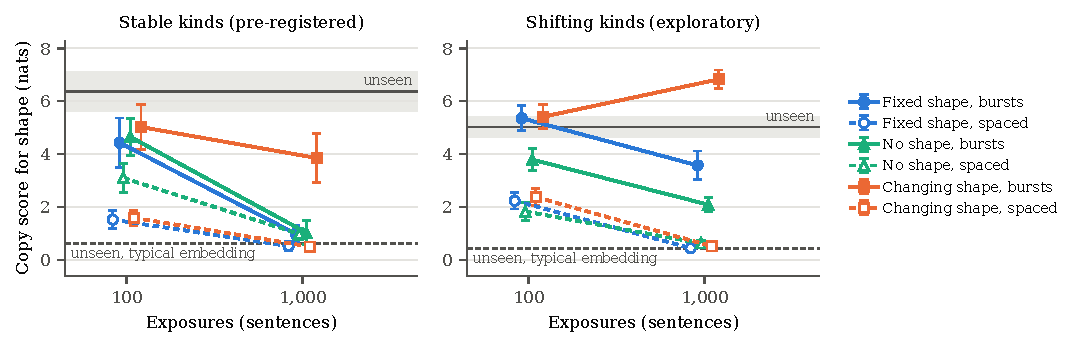
\includegraphics[width=\textwidth]{figures/fig_a10.pdf}
\caption{Experiment 2: copy score by history (colour) and presentation (solid: bursts; dashed: spaced) at 100 and 1,000 exposures, in stable-kind (left, pre-registered tests) and shifting-kind (right, exploratory) corpora (means over ten seeds, sizes averaged; 95\% intervals). Solid line and band: unseen nouns; dashed line: unseen nouns with a typical embedding.}
\label{fig:a10}
\end{figure}

\begin{figure}[!htbp]
\centering
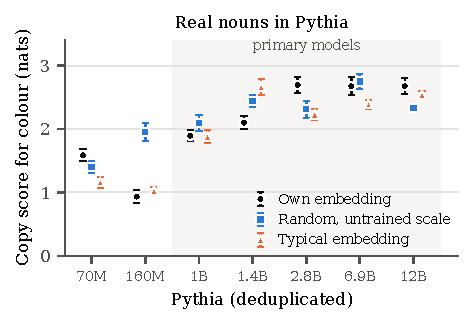
\includegraphics[width=0.6\textwidth]{figures/fig_pythia.pdf}
\caption{Copy score for colour of real nouns in Pythia models, with their own input embeddings or replaced ones (means over 44 nouns, 95\% intervals). The registered tests used the 1B to 12B models; 70M and 160M are descriptive.}
\label{fig:pythia}
\end{figure}

\begin{figure}[!htbp]
\centering
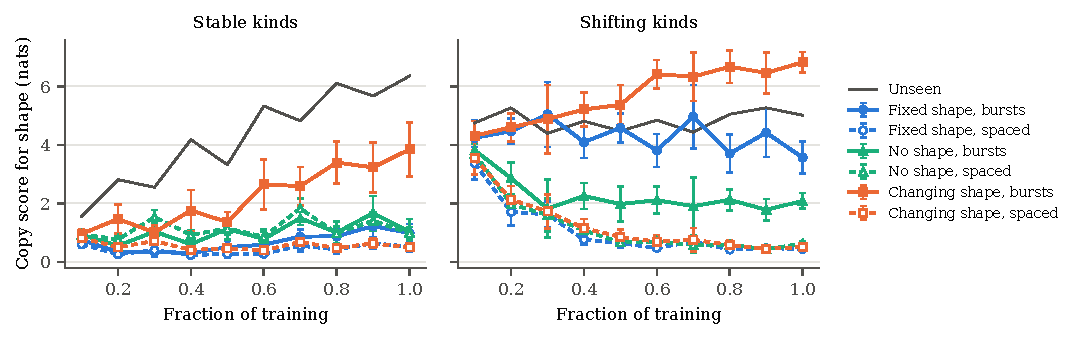
\includegraphics[width=\textwidth]{figures/fig_a10_formation.pdf}
\caption{Experiment 2. Copy score over training for nouns with 1,000 exposures, by history and presentation, and for unseen nouns (exploratory; saved weights every 1,000 steps; means over ten seeds, sizes averaged; 95\% intervals). A noun with 1,000 exposures has had about 1,000 $\times$ ($t - 0.05$)/0.9 sentences by fraction $t$ of training, so exposure and training time rise together. The unseen-noun line zig-zags by 1 to 2 nats because the three sizes save weights at different fractions of training and differ in level.}
\label{fig:a10formation}
\end{figure}

\FloatBarrier
\section{Experiment 3 (Amendment 11)}\label{app:O}
\setcounter{table}{0}\renewcommand{\thetable}{\thesection\arabic{table}}
\textbf{Registration.} Amendment 11 is Experiment 3. It was registered in the project's public OSF record (link withheld for review) after all results of Experiment 2 and its exploratory analyses, after its corpora were built and checksummed, and before any of its models was trained (apart from deleted 100-step pipeline checks), to test the exploratory findings of Experiment 2 on new models. Part A repeated the stable-kind design of Experiment 2 with ten new seeds at 3.4M, 10.9M and 25.6M parameters (30 models). Part B trained ten models of 85.6M parameters (12 layers, 12 heads, width 768) on the same corpora as the 25.6M models. Part C trained five seeds at each of the three smaller sizes on corpora in which all 36 familiar nouns had changing shapes (pure\_changing) or all had fixed shapes (pure\_fixed), nine nouns per cell, with the same exposures and share of text as the mixed design (30 models). The assignment of noun forms to cells follows the Experiment 2 rule by seed position; model weights, reading order and placement are new. All 40 corpora passed a checker and matched checksums recorded before training. Registered rules for failed models (non-finite loss, or a final loss more than 0.5 nats above the median of its size and design) and for complete seeds were applied; no model failed. Part A used Holm correction over H50, H51, H52 (difference), H53, H55 and H56, with direction required at two of three sizes; equivalence tests used two one-sided tests against $\pm$0.3 nats. H55 is a seed-level test: within each model, the copy scores of the 18 familiar nouns at 1,000 exposures were regressed on the embedding's cosine with its initial value, its relative distance from the trained kinds' mean embedding, its norm and a changing-burst indicator, and the indicator's coefficient was averaged over sizes within seed. The 85.6M models were trained on an Apple M3 Ultra (MPS, PyTorch 2.14.1), the others on the machine used for Experiment 2. One deviation: after all 85.6M models had finished, their training loop was started again by mistake and stopped at step 1; only a configuration file was rewritten, with the same content, and no model or score changed.

\begin{table}[!htbp]
\centering\small

\begin{tabular}{@{}l>{\raggedright\arraybackslash}p{0.36\textwidth}rlrc>{\raggedright\arraybackslash}p{0.16\textwidth}@{}}
\toprule
& Test & Estimate & 95\% CI & $p$ & Sizes & Reading \\
\midrule
M3 & Unseen nouns' copy score minus 1 nat (manipulation check; one-sided) & 5.88 & [5.31, 6.45] & $<$.001 &  & Passed \\
H50$^h$ & At 1,000: changing-shape bursts minus fixed-shape bursts (one-sided; primary) & 3.68 & [2.99, 4.37] & $<$.001 & 3 & Supported \\
H51$^h$ & Changing shape: bursts minus spaced, pooled (one-sided) & 4.14 & [3.60, 4.69] & $<$.001 & 3 & Supported \\
H52$^h$ & Spaced: fixed minus changing shape, pooled (two-sided; TOST $\pm$0.3) & \textminus{}0.25 & [\textminus{}0.35, \textminus{}0.15] & $<$.001 & 3 & Different (fixed lower); not equivalent \\
H53$^h$ & Fixed-shape spaced nouns: $L(s^*) - L(s)$, pooled (one-sided) & 5.84 & [5.57, 6.11] & $<$.001 & 3 & Supported \\
H54 & At 1,000: noun-specific copy score of changing-shape bursts (TOST $\pm$0.3) & 0.08 & [0.02, 0.14] & .015 &  & Within $\pm$0.3 \\
H55$^h$ & At 1,000: changing-shape bursts minus embedding-geometry prediction (one-sided) & 3.67 & [3.03, 4.32] & $<$.001 & 3 & Supported \\
H56$^h$ & At 1,000: query-noun minus context-noun effect of changing vs fixed bursts (one-sided) & 1.25 & [0.94, 1.56] & $<$.001 & 3 & Supported \\
M3B & 85.6M models: unseen copy score minus 1 nat (one-sided) & 5.96 & [5.22, 6.69] & $<$.001 &  & Passed \\
H57 & 85.6M models, at 1,000: changing-shape bursts minus fixed-shape bursts (one-sided) & 4.18 & [2.95, 5.41] & $<$.001 &  & Supported \\
M3C & Changing-only corpora: unseen copy score minus 1 nat & 5.16 & [3.25, 7.08] & $<$.001 &  & Passed \\
M3C & Fixed-only corpora: unseen copy score minus 1 nat & 3.87 & [2.84, 4.90] & $<$.001 &  & Passed \\
H58 & At 1,000: changing-shape bursts (changing-only) minus fixed-shape bursts (fixed-only) (one-sided) & 5.51 & [4.24, 6.78] & $<$.001 & 3 & Supported \\
H59 & At 1,000: changing-shape bursts, changing-only minus mixed corpora (two-sided; TOST $\pm$0.3) & 0.24 & [\textminus{}1.44, 1.92] & .712 &  & Inconclusive \\
H59 & At 1,000: fixed-shape bursts, fixed-only minus mixed corpora (two-sided; TOST $\pm$0.3) & \textminus{}1.00 & [\textminus{}1.20, \textminus{}0.80] & $<$.001 &  & Lower in fixed-only corpora \\
\bottomrule
\end{tabular}
\par\smallskip\parbox{\textwidth}{\footnotesize H52: TOST $p$ = 0.14; 90\% interval [\textminus{}0.33, \textminus{}0.17]. H54: TOST $p$ $<$.001. H55, pooled noun-level regression with size and seed effects and seed-clustered errors: 3.82 [3.18, 4.46]; without no-shape nouns: 3.66 [3.05, 4.28]. H55 by size (per-model regression): 6.36, 2.47, 2.19.}
\caption{Registered tests of Experiment 3 (seed-level estimates, nats; sizes averaged within seed; t-based 95\% intervals). Holm $p$: adjusted over the six Part A tests marked $^h$; other $p$ values are unadjusted. Sizes: number of the three sizes with the estimate's direction.}
\label{tab:O1}
\end{table}

\begin{table}[!htbp]
\centering\small

\begin{tabular}{@{}lrrrrrrr@{}}
\toprule
Context $\backslash$ query & \shortstack{Unseen} & \shortstack{Fixed\\ spaced} & \shortstack{Fixed\\ bursts} & \shortstack{No shape\\ spaced} & \shortstack{No shape\\ bursts} & \shortstack{Changing\\ spaced} & \shortstack{Changing\\ bursts} \\
\midrule
Unseen & 6.87 & 0.67 & 0.97 & 0.99 & 1.16 & 0.51 & 2.98 \\
Fixed, spaced & 3.47 & 0.54 & 0.89 & 0.73 & 0.90 & 0.48 & 1.90 \\
Fixed, bursts & 5.23 & 0.71 & 1.13 & 0.94 & 1.16 & 0.60 & 3.02 \\
No shape, spaced & 4.12 & 0.40 & 0.85 & 0.83 & 1.00 & 0.41 & 1.82 \\
No shape, bursts & 4.84 & 0.61 & 0.94 & 0.87 & 0.87 & 0.51 & 2.71 \\
Changing, spaced & 4.08 & 0.47 & 0.91 & 0.93 & 1.08 & 0.56 & 2.16 \\
Changing, bursts & 7.09 & 0.81 & 1.28 & 1.32 & 1.44 & 0.80 & 4.73 \\
\bottomrule
\end{tabular}

\caption{Experiment 3, mixed design, 1,000 exposures: copy score when the context sentence is about a noun of one history (rows) and the query names a different noun of the same or another history (columns); means over ten seeds, sizes averaged (24 items per pair and model). Every item names a different noun in the query, so the diagonal is not comparable with the same-noun copy scores of Table~\ref{tab:O2}.}
\label{tab:O3}
\end{table}

\textbf{Mechanism (exploratory, added after the results).} Three analyses of the 30 mixed-design models (scripts/a11\_mechanism.py). \emph{Steering}: in each model, the direction $v$ is the mean input embedding of changing-shape bursts minus that of fixed-shape bursts at one exposure level; it is added to the embeddings of other nouns and the registered items are scored. The direction from 1,000-exposure bursts is applied to spaced and no-shape nouns at 1,000 exposures and to unseen nouns with a typical embedding; the direction from 100-exposure bursts is added to fixed-shape bursts at 1,000 and subtracted from changing-shape bursts at 1,000, so the direction never comes from the nouns it is applied to. The control is a random vector of the same length (Table~\ref{tab:O4}). \emph{Activation patching}: for each fixed-shape burst noun F and the changing-shape burst noun R of the same index (1,000 exposures), the residual stream after a given block at the query noun's position, or at the last position, is copied from the item that names R in the query into the item that names F, and the reverse. After the first block, patching the query noun's position carried 5 to 58\% of the difference between the two items (by size and direction) and patching the last position 47 to 96\%; after the second block, the noun's position carried none and the last position all of it. \emph{Attention}: first-block attention from the last position to the context's shape word, mean over heads, was 0.069 [0.048, 0.089] higher for changing- than fixed-shape bursts at 1,000 exposures and tracked the copy score: across the 12 history-by-exposure cells within each model, Spearman correlations averaged 0.80 [0.76, 0.85] over seeds (0.91, 0.79 and 0.72 by size); pooled over conditions and models, 0.73, and in later layers $-$0.36 to 0.23. Full results: results/amendment11/MECHANISM.md in the supplementary material.

\textbf{Natural text (exploratory, added after the results).} To ask which regime natural text resembles, we counted the 44 nouns of the pretrained test in WikiText-103 (raw training split; 29,433 articles, 83.7 million words; scripts/natural\_regime.py). Of a noun's mentions, a median 40\% (colour-typical nouns) and 24\% (colour-variable) were followed by another mention within 128 words, against a median 0.3\% and 0.1\% expected if mentions were spread evenly (under 1\% for 42 of the 44 nouns; median ratios 133 and 221). We took a basic colour word immediately before the noun as a colour mention (2,341 for colour-typical nouns, 736 for colour-variable). Within an article, two colour mentions of the same noun named the same colour with median agreement 0.98 and 0.86 (nouns with at least three within-article pairs: 13 and 9); two mentions drawn from the whole corpus agreed with probability 0.46 and 0.37 (medians over nouns). Many colour--noun pairs are parts of names (\emph{Black Sea}, \emph{Blue Velvet}), which inflates agreement within articles, so these figures are rough. Per-noun values: results/natural\_regime.csv in the supplementary material.

\textbf{Tied embeddings (exploratory, added after the results).} Ten 3.4M models were trained on the mixed-design corpora of Experiment 3, with the same seeds and settings but with input and output embeddings tied (Apple M3 Ultra; in all ten final models the input and output matrices were identical). With tied embeddings an unseen noun's embedding receives gradient as an output. Seed-level values, with the untied 3.4M models of Experiment 3 in brackets: unseen nouns copied 3.96 [2.43, 5.49] (8.96), and 0.02 [\textminus{}0.18, 0.21] with a typical embedding (\textminus{}0.19); at 1,000 exposures changing-shape bursts copied 1.90 [1.20, 2.60] more than fixed-shape bursts (6.36); changing-shape bursts copied 2.36 [1.47, 3.25] more than changing-shape spaced nouns, pooled (7.09); fixed- minus changing-shape spaced nouns, pooled, was \textminus{}0.01 [\textminus{}0.30, 0.28] (\textminus{}0.23); and fixed-shape spaced nouns preferred their own shape to the context's by 4.61 [4.10, 5.11] (6.94). Familiar nouns of the other five histories kept more copying than in untied models (1.4 to 2.9 nats at 1,000 exposures, against 0 to 0.7), while changing-shape bursts kept less (4.29 against 7.05).


\FloatBarrier
\section{Control: Redrawn and Half-Kept Bursts}\label{app:P}
\setcounter{table}{0}\renewcommand{\thetable}{\thesection\arabic{table}}
\textbf{Status.} Added after the results of Experiments 1 to 3. It was specified before training but not registered. Its design, analysis and predictions were written down and committed to the project repository before any of its models was trained, and its 20 corpora were built and checksummed before training; the training machine rebuilt them and matched every checksum.

\textbf{Design.} As Experiment~3's stable-kind mixed design (same 40 nouns, base text, frames, placement, tokenizer, ten seeds and three sizes; same corpus builder), with six familiar conditions of three nouns each at 100 and 1,000 exposures, plus four unseen nouns: fixed shape spaced and in bursts; changing shape spaced and in bursts; \emph{redrawn-shape bursts}, whose shape is drawn from the corpus's shape distribution for every sentence (the sentences of changing-shape spaced nouns, grouped in fours); and \emph{half-kept bursts}, whose first sentence draws a shape and each later sentence keeps the previous shape with probability 0.5, else draws again. All shapes appear in frame 1. The share of burst sentences whose shape repeats the previous sentence's was 1.00 for changing-shape and fixed-shape bursts, 0.535 to 0.565 for half-kept bursts and 0.091 to 0.113 for redrawn bursts across corpora (chance: 0.102). Thirty models (3.4M, 10.9M, 25.6M; ten seeds) were trained as in Experiment~3 and scored with the same items. All passed the model check (final loss 0.36 to 0.42). One 25.6M model was interrupted by a computer restart and retrained from the start.

\textbf{Analysis.} Primary contrast, fixed in advance: changing-shape minus redrawn-shape bursts at 1,000 exposures, seed-level (sizes averaged within seed), t-based 95\% interval. Useful context predicts a positive difference and redrawn-shape bursts near changing-shape spaced nouns; recurrence predicts no difference.

\textbf{Results.} Table~\ref{tab:P1}. The primary contrast was 3.33 nats [2.74, 3.92], positive in all ten seeds and at every size (5.82, 2.04, 2.14 at 3.4M, 10.9M, 25.6M). Redrawn-shape bursts at 1,000 exposures copied 0.07 [$-$0.01, 0.15] more than changing-shape spaced nouns, and half-kept bursts fell between redrawn and changing-shape bursts at both levels. At 100 exposures redrawn-shape bursts kept some copying (0.96 above spaced). Fixed-shape bursts at 1,000 copied 0.32 [0.18, 0.47] more than redrawn-shape bursts. Unseen nouns copied 4.92 [4.59, 5.25].



\end{document}
